\documentclass[12pt, a4paper, twoside]{report}
\usepackage[utf8]{inputenc}
\usepackage{blindtext}
\usepackage[margin=2cm]{geometry}
\usepackage{markdown}
\usepackage[hyperref]{xcolor}
\usepackage{setspace}
\usepackage{newpxtext}
\usepackage{newpxmath}
\usepackage[margin=1cm, labelfont=bf]{caption}
\usepackage{subcaption}
\usepackage{booktabs}
\usepackage{numprint}
\usepackage{inconsolata}
\usepackage{mathtools}

\usepackage{graphicx}
\linespread{1.5}
\usepackage{xspace}
\usepackage{tikz-feynman}

% Biblatex
\usepackage[sorting=none]{biblatex}
\bibliography{bibliography}

% Hyperlinks
\definecolor{blue1}{RGB}{50, 142, 237}
\definecolor{red1}{RGB}{239, 83, 138}
\definecolor{orange1}{RGB}{243,109,33}
%\usepackage[colorlinks=true, allcolors=blue1]{hyperref}
\usepackage[colorlinks=true, allcolors=orange1]{hyperref}
\usepackage{soul}
\usepackage{amsmath}
\usepackage{bm}
\usepackage{marginnote}
\usepackage{adjustbox}
\usepackage{diagbox}
%\usepackage{svg}

\usepackage{sepfootnotes}

%\usepackage[group-separator={,},separate-uncertainty=true]{siunitx}
\usepackage[separate-uncertainty=true]{siunitx}
\DeclareSIUnit\clight{\text{\ensuremath{c}}}


% Acronyms
\usepackage[acronym,nonumberlist]{glossaries}
\renewcommand*{\glstextformat}[1]{\textcolor{black}{#1}}
%\makeglossaries
\newacronym{COMET}{COMET}{Coherent Muon-to-Electron Conversion}

% Path of figures for each chapter
%\graphicspath{{introduction/}{chapter2/}{conclusion/}}

%
\newcommand{\diff}[2]{\frac{\textrm{d}{#1}}{\textrm{d}{#2}}}

% If table of contents goes too deep, we can limit depth.
%\setcounter{tocdepth}{0}

% Color scheme: 
%https://coolors.co/0081a7-00afb9-fdfcdc-fed9b7-f07167

\begin{document}

% % Title page
% \thispagestyle{empty}
% 
\includegraphics[width=0.4\textwidth]{IMP_ML_1CS_4CP.eps}
% \vfill
% \begin{center}
    
%     {\huge Thesis Title}
    
%     \rule{7cm}{1pt}
%     \vspace{2cm}
    
%     {\Large Matthias Dubouchet}
%     \vspace{1cm}
    
%     {\Large Department of High Energy Physics
    
%     Imperial College London}
%     \vspace{3cm}
    
%     {\large Submitted in partial fulfilment of the requirements\\for the degree of Doctor of Philosophy}
    
% \end{center}

% \vfill
% \clearpage

% % Blank page
% \shipout\null

% \pagenumbering{roman}

% \chapter*{Abstract}


COMET is a future high-precision experiment searching for charged lepton flavour
violation through the muon-to-electron conversion process. It aims to push the
intensity frontier of particle physics by coupling an intense muon beam with
cutting-edge detector technology. The first stage of the experiment, COMET
Phase\nobreakdash-I, is currently being assembled and will soon enter its data acquisition
period. It plans to achieve a single event sensitivity to $\mu$--$e$ conversion
in aluminium of $3.1 \times 10^{-15}$.

This thesis presents a study of the sensitivity and backgrounds of \mbox{COMET
Phase\nobreakdash-I} using the latest Monte Carlo simulation data produced. The background
contribution from cosmic ray-induced atmospheric muons is estimated using a
backward Monte Carlo approach, which allows computational resources to be
focused on the most critical signal-mimicking events.

Analysis of a $\mu$--$e$ conversion simulation sample suggests that COMET
Phase\nobreakdash-I will reach a single event sensitivity of $3.6 \times 10^{-15}$ within 146
days of data acquisition. In that period, the background contribution from
atmospheric muons is estimated to be 0.08 events under optimistic conditions,
namely a \SI{99.99}{\percent}-efficient Cosmic Ray Veto system and
\SI{99}{\percent} muon identification rate by the main detector.

% 
\chapter*{Declaration}
This dissertation is the result of my own work except where explicit reference
is made to the work of others. In addition, the methods and results reported in
Section~\ref{sec:quality_metrics} were investigated by a pair of MSci students
with my guidance.

\hfill Matthias Dubouchet

\vspace{2cm}
The copyright of this thesis rests with the author. Unless otherwise indicated, 
its contents are licensed under a Creative Commons Attribution-Non 
Commercial 4.0 International Licence (CC BY-NC). 
Under this licence, you may copy and redistribute the material in any medium 
or format. You may also create and distribute modified versions of the work. 
This is on the condition that: you credit the author and do not use it, or any 
derivative works, for a commercial purpose. 
When reusing or sharing this work, ensure you make the licence terms clear to 
others by naming the licence and linking to the licence text. Where a work has 
been adapted, you should indicate that the work has been changed and 
describe those changes. 
Please seek permission from the copyright holder for uses of this work that are 
not included in this licence or permitted under UK Copyright Law.

% \tableofcontents
% \printglossary[type=\acronymtype]
% \clearpage

% \pagenumbering{arabic}

\tableofcontents

%\chapter{The COMET Experiment}\label{ch:comet}

% \begin{markdown}
% ---

% - Description of the COMET experiment's goal, design with nice illustrations
%     + Signal and background:
%         + mu-e conv signal description
%         + **List of background sources**
% + CyDet:
%     + For simulation section, need to explain how CDC and CTH work, and how
%       combined they enable mu--e conv measurement
%     - Detailed description of the CDC, which is crucial for the GAN section.
%      - Stereo angles
% + Phase alpha?

% - References: TDR, SINDRUM II, 

% ---

% + Requirements: high sensitivity to signal, efficient rejection of backgrounds
%  + -> Need intense muon beam, pulsed, and detector design must avoid
%    backgrounds
% + TIMING of signal (muon lifetime)
% + Proton beam energy: why 8 Gev -> antiproton production
% + Intensity: beam current, beam power, POTs per second
% + Send backward-going secondaries to detector, discard the main part of
%   secondaries (forward-going)
% + Curved solenoid + dipole field (by tilting coils, see Krikler)
% + Stopping target -> why Al
% + Bunch structure, extinction
% + Phase-I detectors: StrECAL and CyDet

% ---
% \end{markdown}

% Description and goals
COMET (COherent Muon-to-Electron Transition) is a future muon-beam experiment
designed to search for the muon-to-electron conversion
process~\cite{the_comet_collaboration_comet_2020}. It is currently under
construction at the Japan Proton Accelerator Research Complex (J-PARC) facility
in Tokai, Japan. The goal of COMET is to be \numprint{10000} times more
sensitive to $\mu$--$e$ conversion than the current world-leading limit set by
the SINDRUM II experiment~\cite{Bertl:2006up}. 

\subsubsection{Requirements}
In order to reach its goal, the COMET experiment is designed with strict
requirements defined to make the conversion signal as clear as possible, while
efficiently rejecting background events. The essential requirements that define
the COMET experiment are:
\begin{itemize}
    \item An intense muon source to probe the rare conversion process;
    \item A pulsed beam such that timing information can be used to reject
    backgrounds;
    \item Strict selection of charge and momentum of beam particles prior to
    reaching the detector;
    \item A tracking detector to search for the \SI{104.97}{\MeV} conversion
    signature.
\end{itemize}
These requirements and the design choices that were made to address them are
described in more detail in the rest of this chapter.

\subsubsection{Strategy}
COMET is planned to run in a staged approach such that the properties of the
newly designed beam can be finely understood before making the measurement.
COMET Phase-I has a double purpose, each fulfilled by a distinct detector
system. The StrECAL detector, composed of a straw-tube tracker and
electromagnetic calorimeter, will study the beam composition and timing
properties and increase our understanding of potential backgrounds. The
Cylindrical Detector, composed of a cylindrical drift chamber and a trigger
hodoscope, will be used to perform a $\mu$--$e$ conversion search with a
single-event sensitivity (see Section~\ref{sec:SES}) of $3\times 10^{-15}$, a
factor-100 improvement over SINDRUM II. COMET Phase-II is a planned upgrade to
Phase-I with higher beam intensity and better background rejection via a longer
momentum-selecting beamline. Phase-II aims to improve on the single-event
sensitivity of Phase-I by another factor $100$ to reach a single event
sensitivity of $2.6\times 10^{-17}$.

\subsubsection{Design}
Figure~\ref{fig:comet_schematic} shows a top-down schematic view of the COMET
experiment, laying out the different sections that make up the beamline in
Phase-I and Phase-II. In the latter, the transport solenoid is doubled to allow
more pions to decay into muons while tightening the momentum selection further.
An additional curved solenoid, the \emph{electron spectrometer,} further
eliminates particles whose momenta do not match the \SI{104.97}{\MeV} conversion
signature before they enter the detector system. While Phase-I will use the
StrECAL to study the beam properties, Phase-II will use it as the
conversion-searching detector system.\\
The following sections describe in more detail each component of the COMET
beamline.

\begin{figure}
    \centering
    \begin{subfigure}[b]{0.46\textwidth}
    \centering
        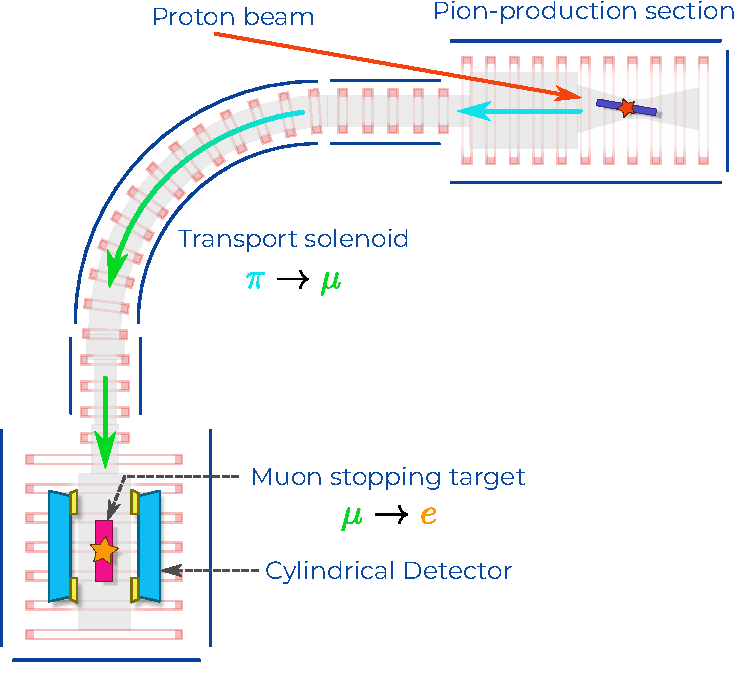
\includegraphics[width=\textwidth]{chapter2/comet_schematic_phase-I.pdf}
        \vspace{3cm}
        \caption{Phase-I with the Cylindrical Detector.}
    \end{subfigure}
    \hfill
    \begin{subfigure}[b]{0.49\textwidth}
        \centering
        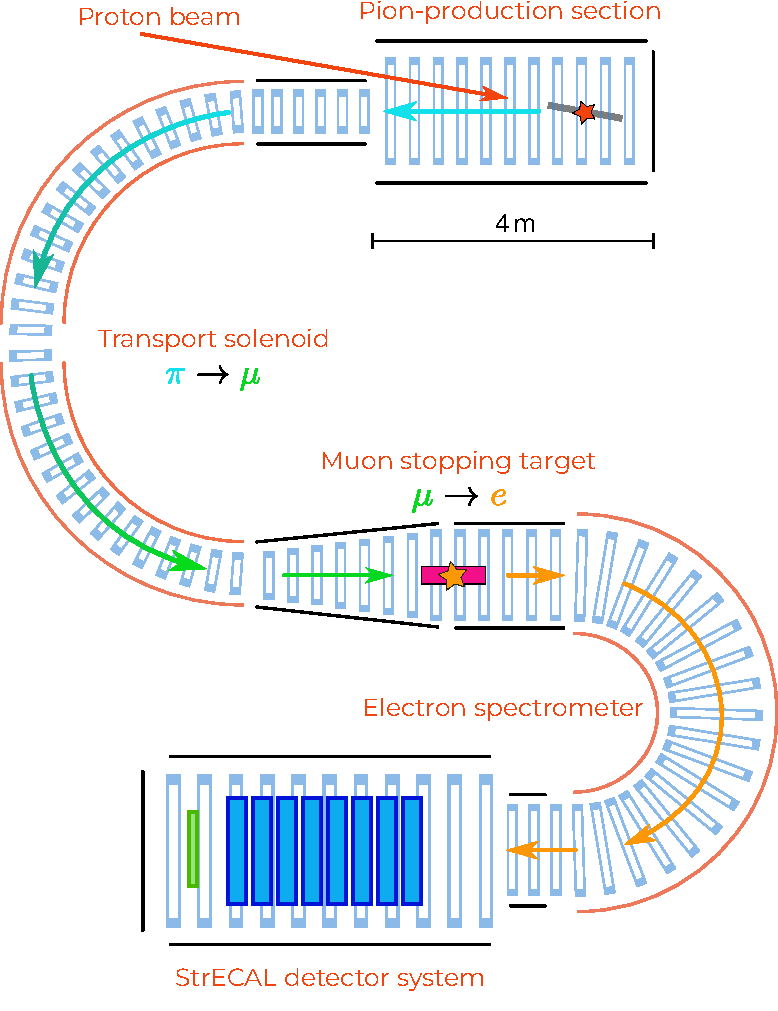
\includegraphics[width=\textwidth]{chapter2/comet_schematic.pdf}
        \caption{Phase-II.}
    \end{subfigure}
    \caption{ Schematic top-down view of the COMET experiment. The beam pipe is
    represented in gray, and the light red rectangles along the beamline
    represent the solenoids that generate the magnetic field. Curved solenoids
    additionally help to select charge and momentum, as discussed in
    Section~\ref{sec:curved_solenoids}.}
    \label{fig:comet_schematic}
\end{figure}



\section{Proton beam}\label{sec:COMET_beam}

Muons in the COMET experiment are produced from the decay of pions created in
proton collisions on a static solid target. The primary proton beam is provided
by the J-PARC facility. Protons are delivered with an energy of \SI{8}{\GeV},
which is picked to maximise the pion yield while minimising the production of
anti-protons, a potential background source.

The timeline of a COMET event is shown in Figure~\ref{fig:timing_distributions}.
The beam has a pulsed time profile: protons are grouped into \SI{100}{\ns}
bunches, each containing $16\times 10^6$ protons. Bunches are separated by
\SI{1170}{\ns}. Just after the collision, secondary particles will quickly move
down the COMET beamline and produce numerous background hits in the detector
system. This prompt and intense flooding of the detector is called the
\emph{beam flash}, and typically dies down within a few hundred nanoseconds.
Muons bound by the muon stopping target have a lifetime of \SI{864}{\ns} (see
Section~\ref{sec:stopping_target}). This, combined with the \SI{1170}{\ns} time
span between two bunches, allows COMET to search for $\mu$--$e$ conversion after
the beam flash has ended, and until the next collision occurs. 

\begin{figure}
    \centering
    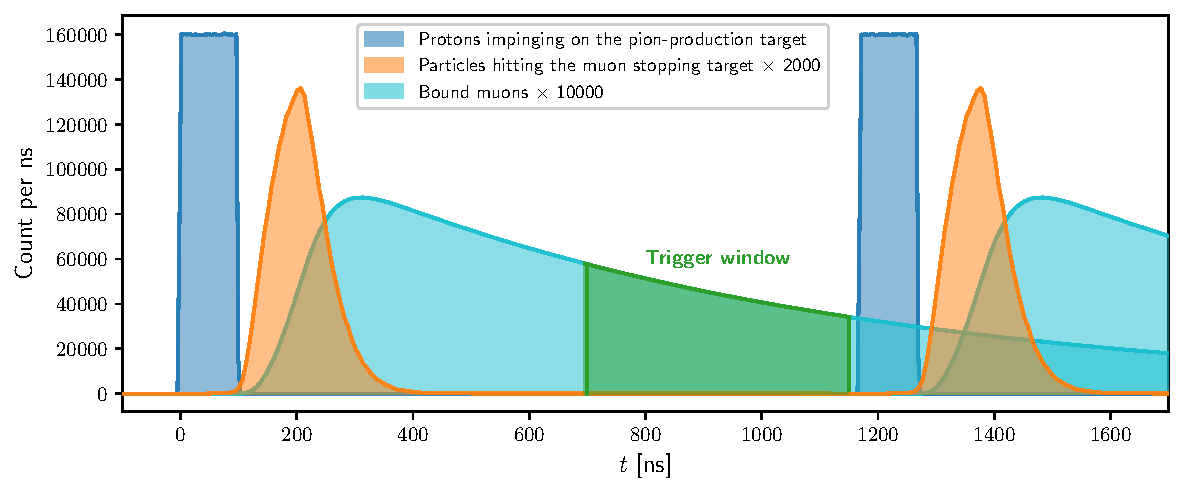
\includegraphics[width=0.85\textwidth]{chapter2/timing_plot_realistic_beam_flash.pdf}
    \caption{ Timeline of a COMET event. Shortly after the proton collision, the
        beam flash floods the detector and muons begin to be bound in the muon
        stopping target. The Phase-I trigger window shown here starts at
        $t=\SI{700}{\ns}$ and lasts until the next proton bunch collision.  }
    \label{fig:timing_distributions}
\end{figure}

% Could also add info on buckets, 4/5 time structure

Stray protons arriving in the time between two bunches can contribute to the
experimental backgrounds by sending particles toward the detector region at
unexpected timings. COMET requires the J-PARC proton beam to have fewer than one
such stray proton for every 600 bunches in order to reach its sensitivity goals.
This corresponds to an extinction factor
\begin{equation}\label{eq:extinction}
R_\mathrm{extinction} \equiv \frac{\mathrm{protons\ between\
bunches}}{\mathrm{protons\ per\ bunch}} \approx 10^{-10}.
\end{equation}

\section{Pion-production section}

\begin{figure}
    \centering
    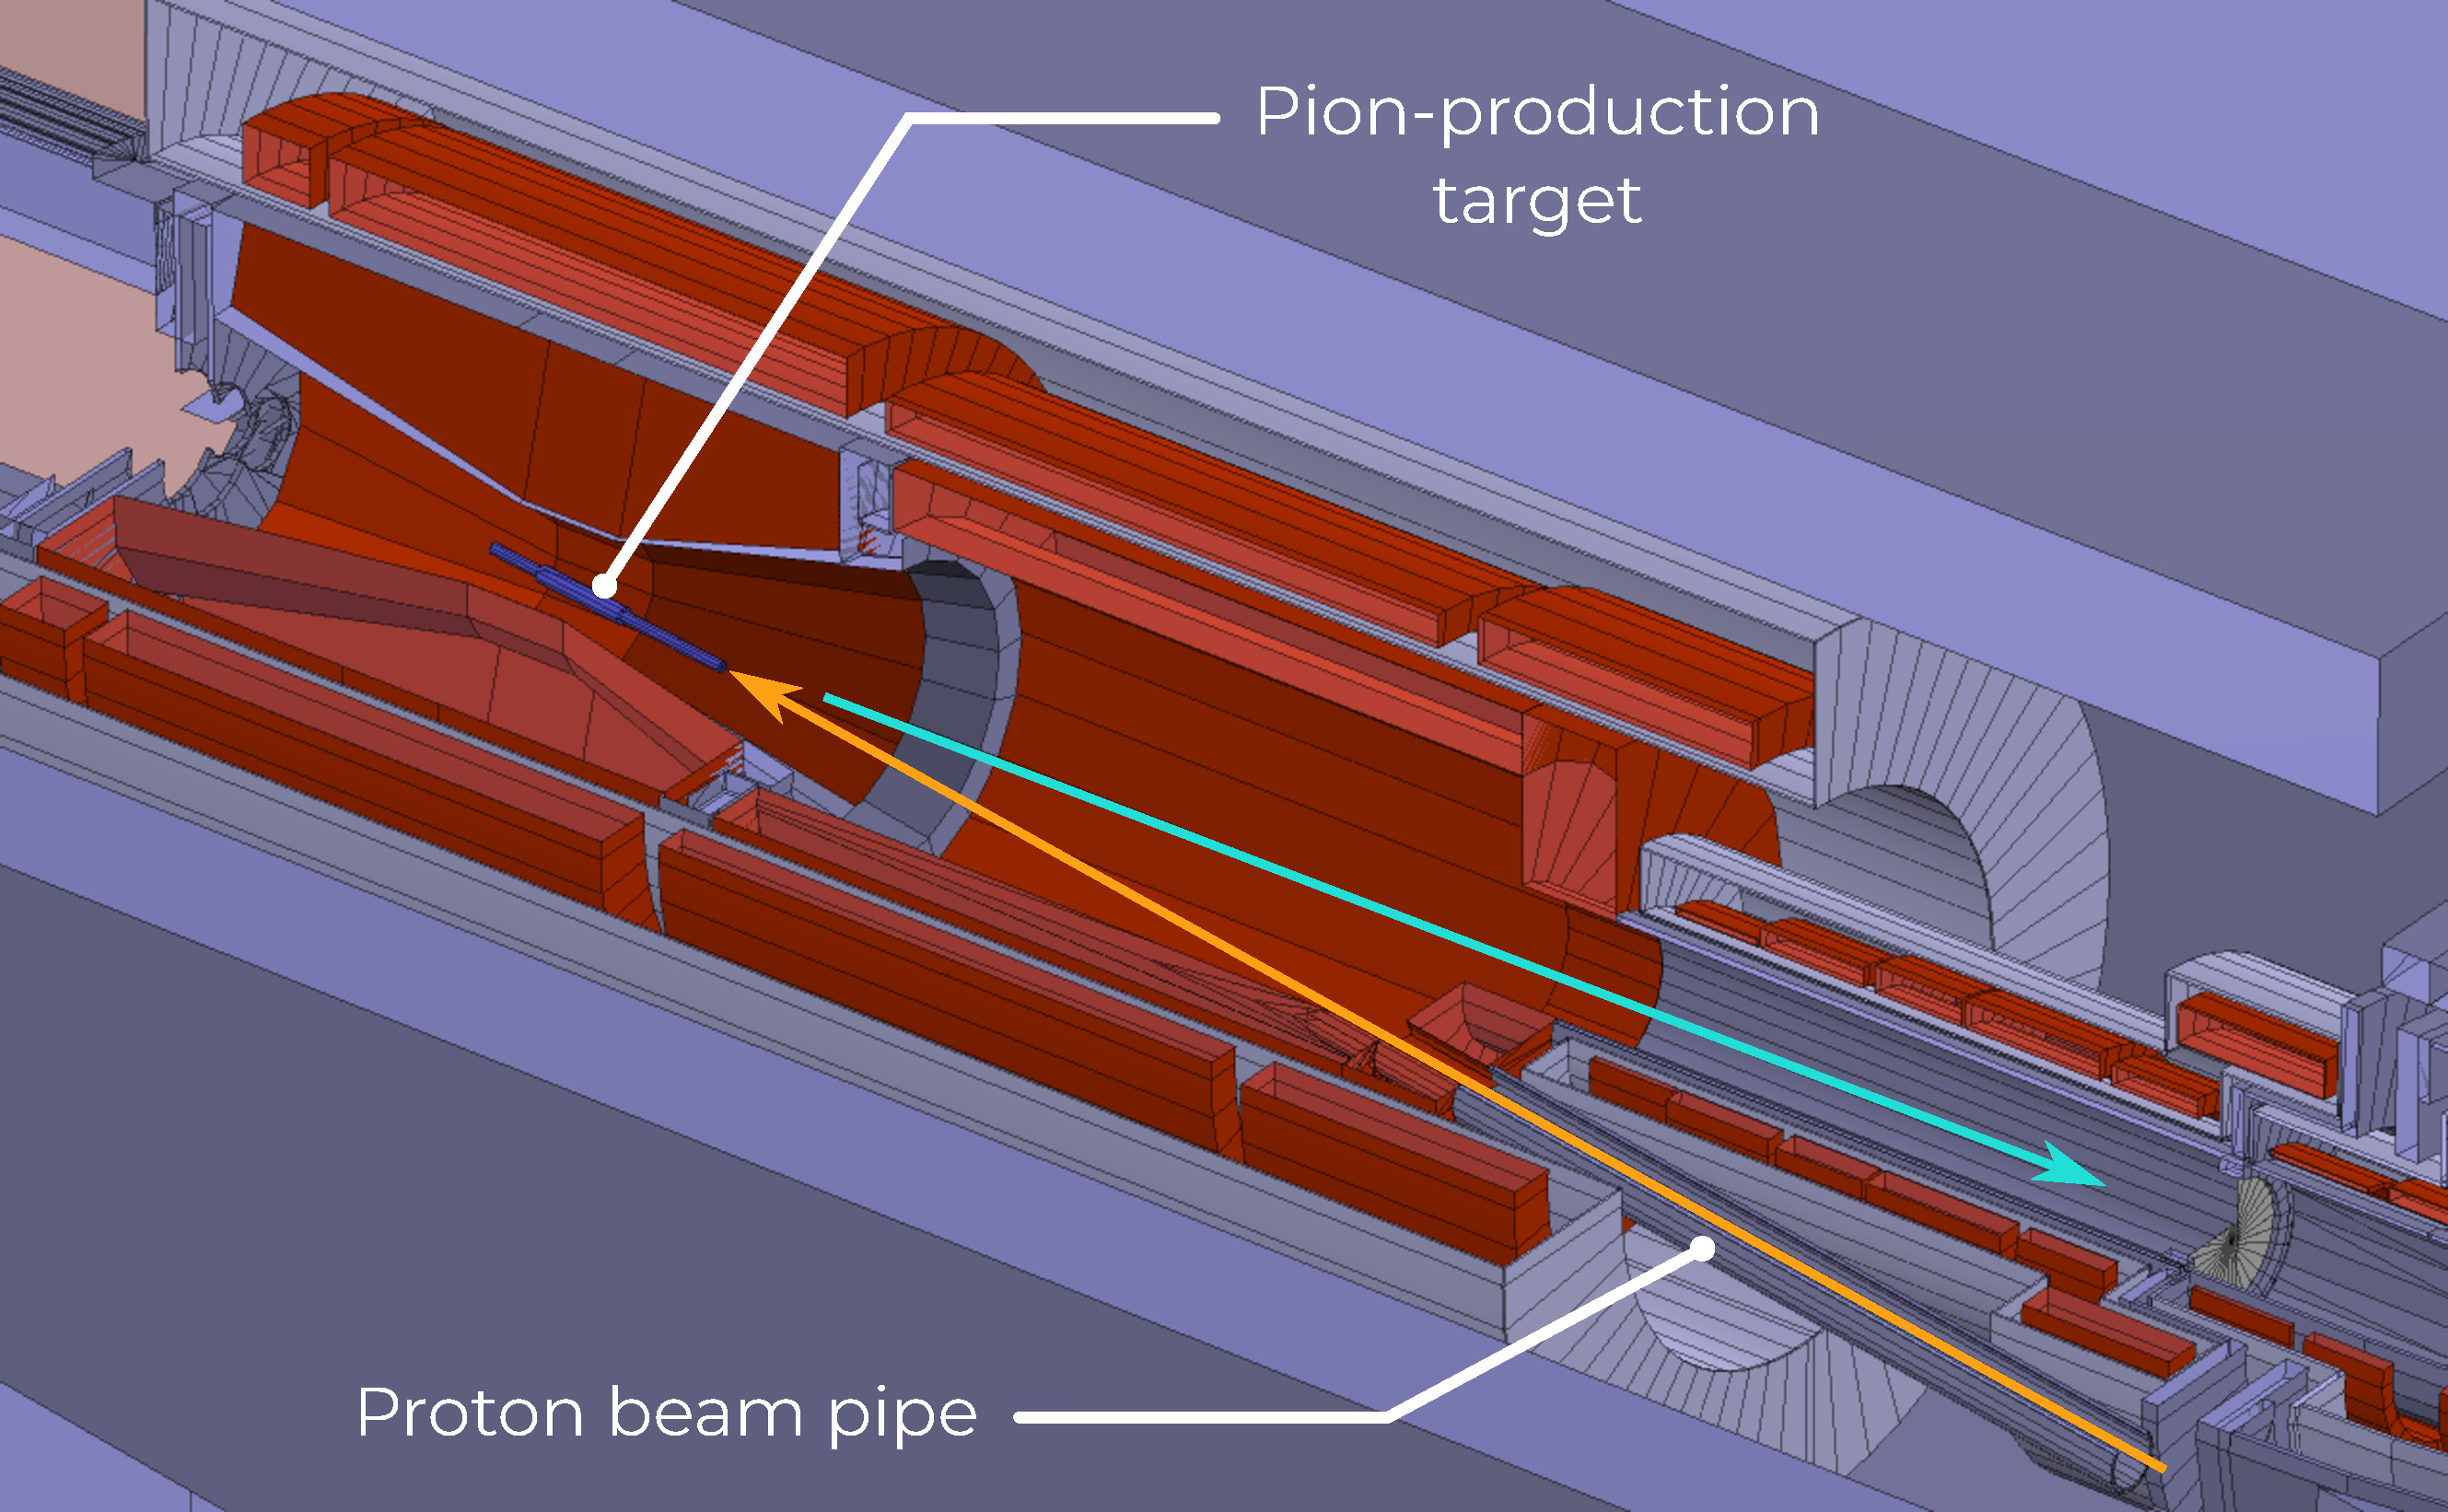
\includegraphics[width=0.8\textwidth]{chapter2/pion_production_section.png.pdf}
    \caption{ Cutaway view of the pion-production section. The orange arrow
        indicates the path of the proton beam while the teal arrow shows the
        direction of backward-going pions captured by the magnetic field.}
    \label{fig:pion_production_section}
\end{figure}

Pions are produced by the collision of the proton beam on a solid target made of
graphite in Phase-I, and tungsten in Phase-II. This region is permeated by a
\SI{5}{\tesla} magnetic field produced by a superconducting solenoid, which
confines the pions and directs them toward the transport solenoid.
Figure~\ref{fig:pion_production_section} shows a cutaway view of this
region.


Pions produced moving backward with respect to the proton beam have a lower
energy than those produced going forward, although they are not as numerous. In
COMET, it is crucial to eliminate high-energy particles in the muon beam that
could produce secondaries mimicking the conversion signal. Hence, the beamline
is positioned in the opposite direction to the proton beam such that only those
low-energy backward-moving pions are allowed into the COMET beamline.
Figure~\ref{fig:pion_momentum} illustrates this by showing that pions moving
backward with respect to the proton beam have a much lower momentum cut-off than
forward-moving pions.

\begin{figure}
    \centering
    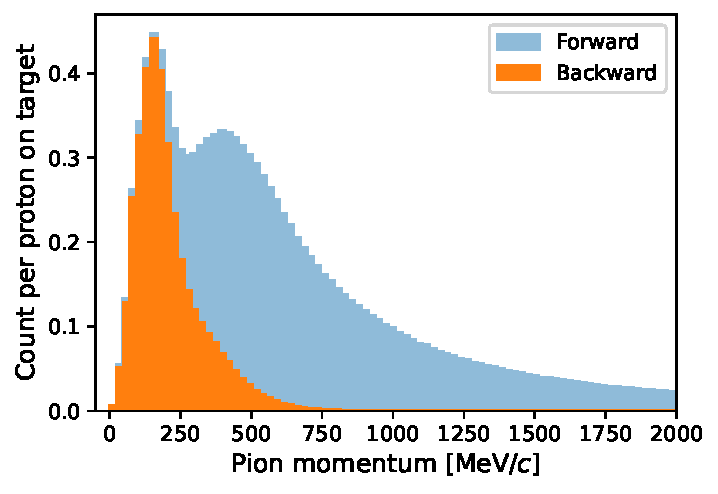
\includegraphics[width=0.5\textwidth]{chapter2/pion_mom-v2.pdf}
    \caption{ Momentum distribution of pions produced by simulating proton
    collisions with Geant4, depending on whether their initial direction is
    forward or backward with respect to the proton beam direction. }
    \label{fig:pion_momentum}
\end{figure}

\section{Transport solenoid}\label{sec:curved_solenoids}

\begin{figure}
    \centering
    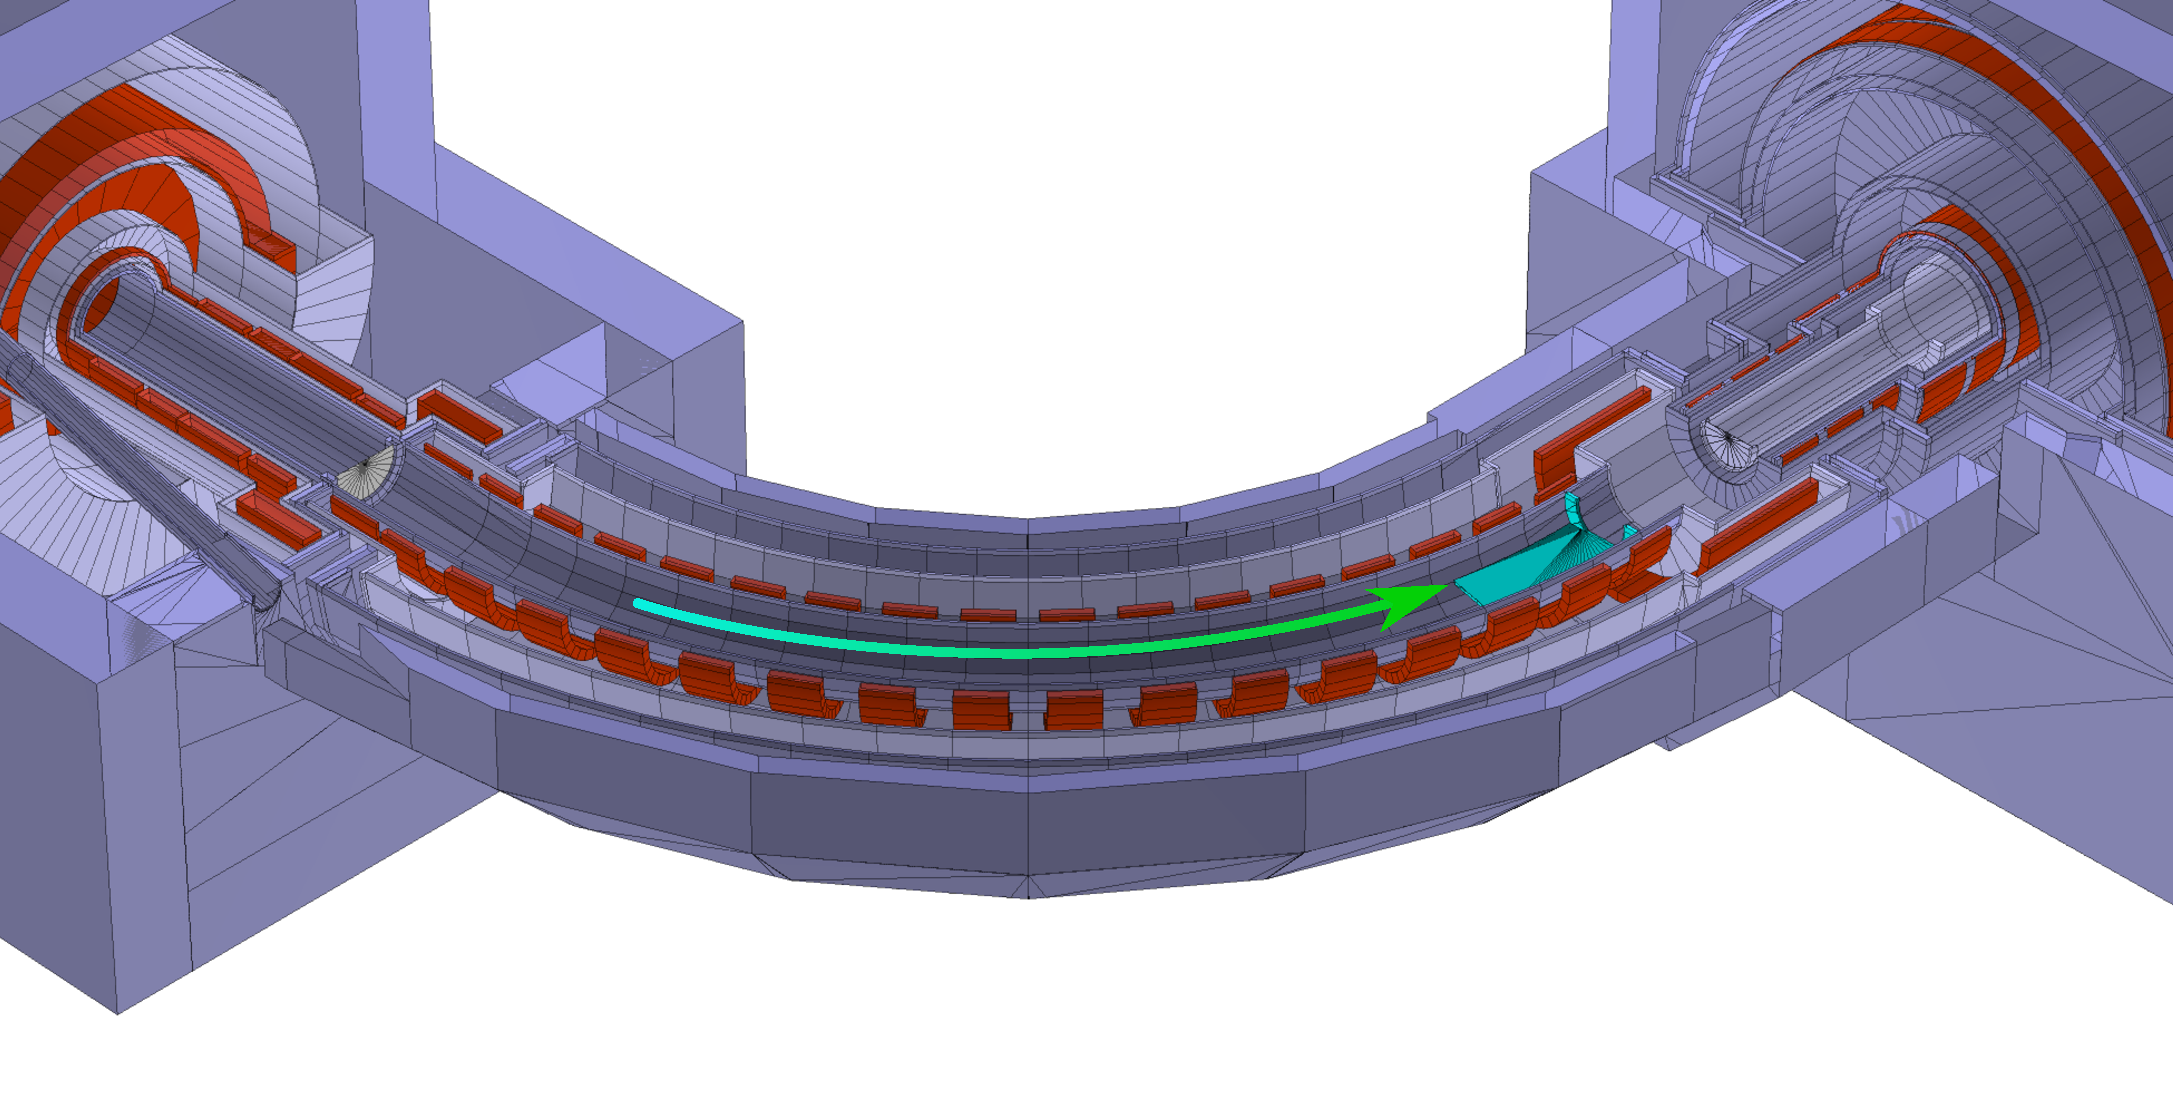
\includegraphics[width=0.8\textwidth]{chapter2/transport_solenoid.pdf}
    \caption{ Cutaway view of the Phase-I transport solenoid. The curved
        solenoid (in red) combined with collimators (in teal) select particles
        depending on their charge and momentum. }
    \label{fig:transport_solenoid}
\end{figure}

The transport solenoid is a curved pipe connecting the pion-production section
to the muon stopping section. Its purpose is twofold. Firstly, it allows a
larger fraction of pions to decay along the length of the beamline. Secondly,
the curved shape combined with its magnetic field and collimators allows it to
select negatively charged particles of a specific momentum. 


The magnetic field of a curved solenoid is slightly stronger on the inside of
the curve than on the outside. Since charged particles follow helical
trajectories, this has the net effect of making them drift vertically and the
amount of drift $D$ depends on momentum $p$ according to the equation
\begin{equation*}
    D = \frac{1}{q B} \frac{s}{R} \frac{2 p^2_L + p^2_T}{2 p_L},
\end{equation*}
where $q$ is the charge, $B$ is the strength of the field along the gyration
axis, $s$ is the distance travelled along the solenoid, $R$ is the radius of the
curve, and $p_L$ and $p_T$ respectively denote momentum longitudinal and
transverse to the solenoid axis~\cite{ben_thesis}. From this expression, one can
see that oppositely charged particles drift in opposite directions, and that
drift is overall stronger for higher-momentum particles. The ratio
$\frac{p_L}{p_T}$, which defines a helical trajectory's \emph{pitch angle}, is
also a major factor in a particle's drift.

\begin{figure}
    \centering
    \begin{subfigure}[b]{0.46\textwidth}
        \centering
        \hspace{-0.8cm}
        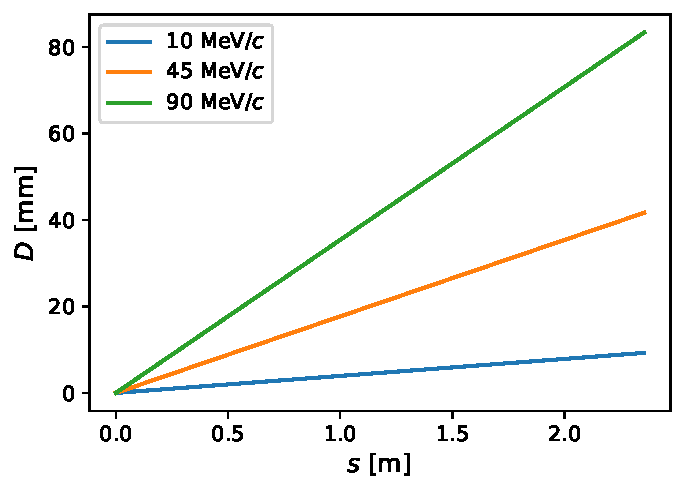
\includegraphics[width=\textwidth]{chapter2/drift_vs_s_0mT.pdf}
        \caption{No dipole field.}
    \end{subfigure}
    \hfill
    \begin{subfigure}[b]{0.46\textwidth}
        \centering
        \hspace{-0.8cm}
        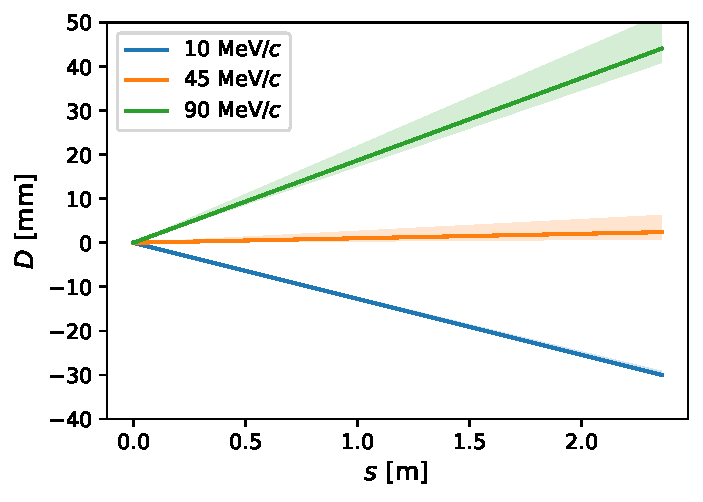
\includegraphics[width=\textwidth]{chapter2/drift_vs_s_0.05mT.pdf}
        \caption{\SI{0.05}{\tesla} vertical dipole field.}
    \end{subfigure}
    \caption{ Effective drift of particles of various momenta as they progress
        along the Phase-I transport solenoid. Solid lines show drift for a pitch
        angle of \SI{45}{\degree}, and the surrounding bands show the effect of
        a $\pm \SI{10}{\degree}$ change in pitch angle on the drift. By applying
        an additional vertical magnetic field, particles of a specific momentum
        can be selected. Here, a \SI{0.05}{\tesla} dipole field allows
        particles around \SI{45}{\MeV/\clight} to stay on axis while higher- and
        lower-momentum particles drift in opposite directions, and can then be
        suppressed by collimators at the end of the transport section. }
    \label{fig:drift}
\end{figure}

The drift caused by the curved solenoid makes all particles of the same charge
move in the same direction to varying degrees depending on momentum. In order to
select particles of a specific momentum, a vertical component is added to the
magnetic field to counterbalance the drift. Selected particles thus stay on
axis, while higher- and lower-momentum particles drift off axis. With the addition
of a collimator at the end of the transport solenoid, particles with unwanted
momenta are effectively eliminated from the beam.

Figure~\ref{fig:drift} shows drift $D$ as a function of $s$, the longitudinal
distance travelled by particles along the solenoid. This illustrates how, by
adding a dipole field, particles with a momentum outside the required range can
be efficiently eliminated by collimators at the top and bottom of the beam pipe.

\section{Muon stopping target}\label{sec:stopping_target}
The purpose of the muon stopping target is to slow down and stop as many muons
as possible while not blocking the path of converted electrons. It is composed
of a series of 17 thin aluminium disks placed in the way of the muon beam. The
disks are \SI{20}{\cm} in diameter, \SI{0.2}{\mm} thick, and separated by
\SI{5}{\cm}. The stopping target is shown in Figure~\ref{fig:cydet}, surrounded
by the Cylindrical Detector.

The more aluminium there is, the higher the number of muons that will be stopped
and allowed to undergo conversion. However, more material also means more energy
lost by electrons flying outward, hence the design of the target optimises
between muon stopping rate and acceptance of conversion electrons by the
detector system.


The material of the stopping target influences the conversion rate, but also the
lifetime of a muon caught in orbit around a nucleus. A heavy target favours the
expected rate of $\mu$--$e$ conversion, however it also causes the nuclear
capture rate to be higher. In COMET, beam bunches are separated by
\SI{1.17}{\ns} and prompt backgrounds typically die off within a few hundred
nanoseconds. A muonic atom with an iron or heavier nucleus has a lifetime less
than \SI{200}{\ns}~\cite{ben_thesis}, which would be too short to allow muons to
stay bound and convert after the beam flash is over. Hence, a light target such
as aluminium, with a longer stopped muon lifetime of
\SI{864}{\ns}~\cite{PhysRevC.35.2212}, is better suited to the COMET conversion
search.

\section{Detector systems}
\subsection{StrECAL}
The StrECAL combines a straw-tube tracking detector with an electromagnetic
calorimeter for energy measurement. In COMET Phase-I, the StrECAL will serve as
a beam characterisation apparatus. It will be placed directly at the end of the
transport solenoid, without a muon stopping target, to study the composition of
the COMET beam and gain a more thorough understanding of potential backgrounds.
The collected data can also serve to validate and refine the Monte Carlo
simulation in preparation for the conversion measurement.

In COMET Phase-II, the StrECAL will serve as the detector system for the
conversion measurement. It will be placed after the electron spectrometer, a
curved solenoid section designed to select conversion electrons, as shown in
Figure~\ref{fig:comet_schematic}. Figure~\ref{fig:strecal} shows a rendering of
the StrECAL detector system in Phase-II.

The Straw Tracker uses thin straw tubes as drift chambers, arranged into
circular planes. A series of stations, each one able to measure the horizontal
and vertical position of a particle, are positioned along the beam direction.
The straws have a resolution better than \SI{100}{\um}, which allows the Straw
Tracker to reconstruct trajectories and estimate particle momenta via
time-of-flight information.

The ECAL is a crystal electromagnetic calorimeter which supplements the Straw
Tracker in measuring energy and thus in identifying electrons. The ECAL uses
lutetium-yttrium oxyorthosilicate (LYSO) as its scintillating crystals and
avalanche photodiodes to collect the emitted photons.


\begin{figure}
    \centering
    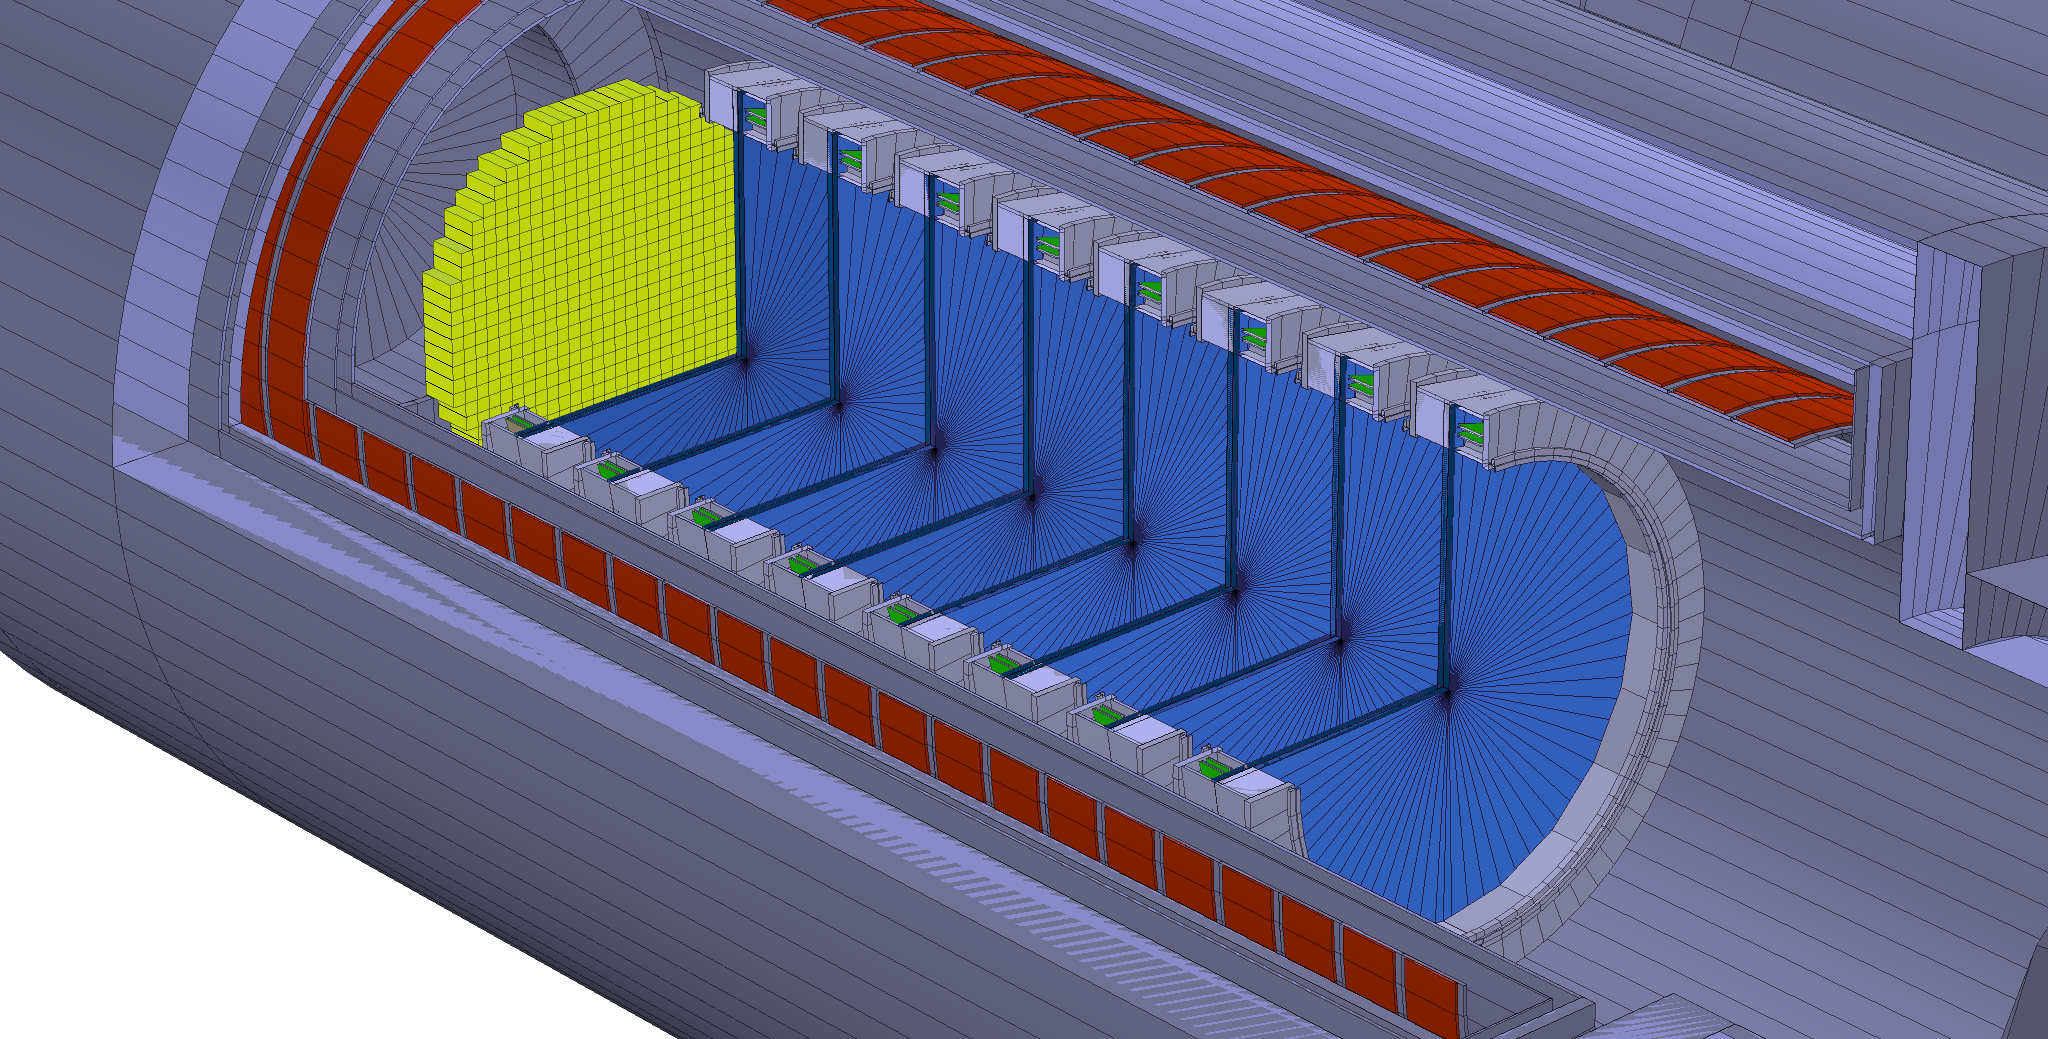
\includegraphics[width=0.8\textwidth]{chapter2/strecal_recolor.png}
    \caption{ Cutaway view of the StrECAL detector. The Straw Tracker stations
    are shown in blue and the ECAL in yellow.  }
    \label{fig:strecal}
\end{figure}

\subsection{CyDet}
The Cylindrical Detector (CyDet) consists of a Cylindrical Drift Chamber (CDC)
for tracking and a Cylindrical Trigger Hodoscope (CTH) for triggering on
specific event signatures. The CyDet surrounds the muon stopping target and sits
within the detector solenoid which generates a \SI{1}{\tesla} longitudinal
magnetic field. This configuration, shown in Figure~\ref{fig:cydet}, is designed
to eliminate backgrounds from the beam itself as well as low-momentum products
of the collision while maximising the acceptance of conversion electrons.
Figure~\ref{fig:cydet_signal_event} additionally shows the signature of a
simulated conversion electron inside the CyDet system.

\begin{figure}
    \centering
    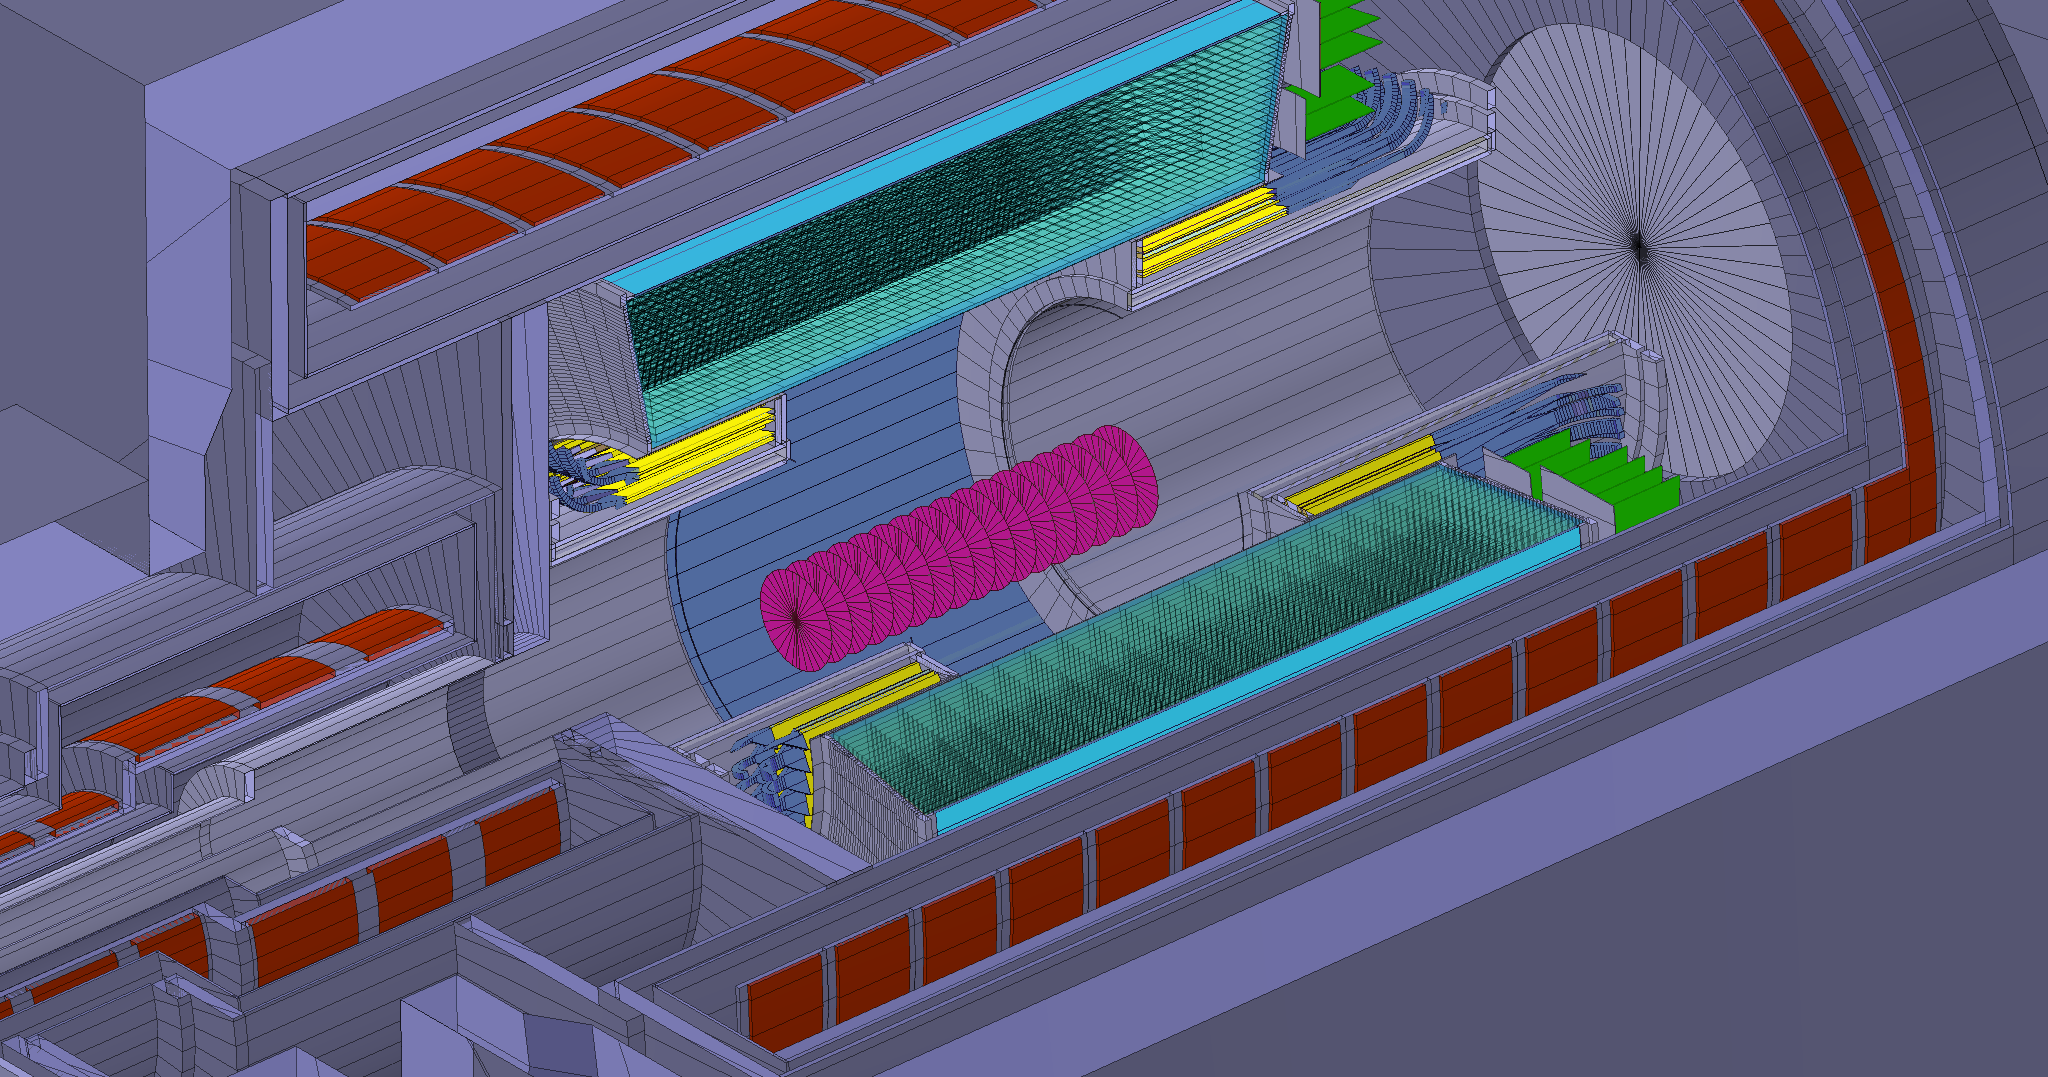
\includegraphics[width=0.8\textwidth]{chapter2/cydet_recolor.png}
    \caption{ Cutaway view of the Cylindrical Detector, composed of the
        Cylindrical Drift Chamber (in teal) and Cylindrical Trigger Hodoscope
        (in yellow). The muon stopping target disks, in purple, sit in the
        centre of the detector system. }
    \label{fig:cydet}
\end{figure}

\subsubsection{Cylindrical Drift Chamber}
The CDC is a drift chamber used to track charged particles emanating from the
muon stopping target. In order to suppress hits from beam particles, the CDC is
wrapped around the beam pipe and has an inner radius of \SI{50}{\cm}. Combined
with the \SI{1}{\tesla} longitudinal magnetic field, this prevents charged
particles with a transverse momentum less than \SI{60}{\MeV/\clight} from
reaching the chamber. In order to achieve the sensitivity goal for Phase-I, the
CDC has a momentum resolution better than \SI{200}{\keV/\clight} in order to
differentiate between conversion electrons and electrons from the high-energy
tails of the decay-in-orbit and radiative muon capture spectra. 

% Geometry
The CDC contains 4986 \emph{sense wires} strung out longitudinally in 20
concentric layers. The wires in each layer are rotated slightly off of the
longitudinal axis, and the rotation is alternatively clockwise and
anti-clockwise from one layer to the next. This special property, called the
\emph{stereo angle}, allows the drift chamber to stereoscopically reconstruct,
within \SI{3}{mm}, the longitudinal position of a particle~\cite{ewen_thesis}. 


% Operating principle
Each sense wire is held at a potential of up to \SI{1900}{\volt} and is
surrounded by 8 grounded \emph{field wires} to generate an inward electric
field. When a charged particle ionises the gas, the field accelerates freed
electrons toward the sense wire. These electrons can gain enough energy to further
ionise the gas, leading to avalanche multiplication (see
e.g.~\cite[Chapter~6]{leo}). The avalanche produces a pulse on the sense wire,
which is acquired by the readout electronics. 


% Drift time

% The time period between the passage of the ionising charged particle and the
% ionisation products inducing a pulse on the wire depends on the \emph{drift
% velocity} of the gas, which depends on the applied voltage.

% ... not necessary?

\subsubsection{Cylindrical Trigger Hodoscope}
The CTH consists of two \emph{modules} that line the inner wall of the CDC, one
upstream and one downstream of the muon stopping target. Each module contains
two layers of 48 partially-overlapping scintillation counters. Each counter has
a time resolution of \SI{1}{\ns}. The main purpose of the CTH is to reject
background events coming from the beam itself and from products of the muon beam
collision while complementing the CDC in identifying conversion electrons.

The overlap between counters allows the CTH to reject a large fraction of
background hits, e.g.\ from photons produced in the muon beam collision. This is
done by only accepting fourfold-coincident events, where four neighbouring
counters (two in the inner layer, two in the outer layer) are hit in a short
\SI{10}{\ns} time span. The CTH thus provides an online triggering mechanism
which significantly reduces the number of background events accepted by the
CyDet system due to its proximity with the muon stopping target.
Figure~\ref{fig:cydet_signal_event} shows how a conversion electron might
produce such a fourfold coincidence.


\subsection{Cosmic ray veto}\label{sec:crv}
The COMET experiment hall is constantly irradiated by muons produced in the
atmosphere by cosmic rays. The cosmic ray veto (CRV) is an additional active
detector which will tightly enclose the CyDet and StrECAL detector systems. Its
purpose is to identify events induced by cosmic muons rather than by the COMET
beam, and thus reduce the probability that such events will be mistaken for a
conversion signal.

\section{Conversion signature}
Conversion electrons are mono-energetic at $E=\SI{104.97}{\MeV}$ and emitted
isotropically by muons stopped in the target disks. In the magnetic field of the
detector solenoid, they have a helical trajectory which can be reconstructed by
the CDC or Straw Tracker. Figure~\ref{fig:cydet_signal_event} shows a simulated
conversion electron going through the Cylindrical Detector.



\begin{figure}
    \centering
    \captionsetup[subfigure]{justification=centering}
    \begin{subfigure}[b]{0.44\textwidth}
    \centering
    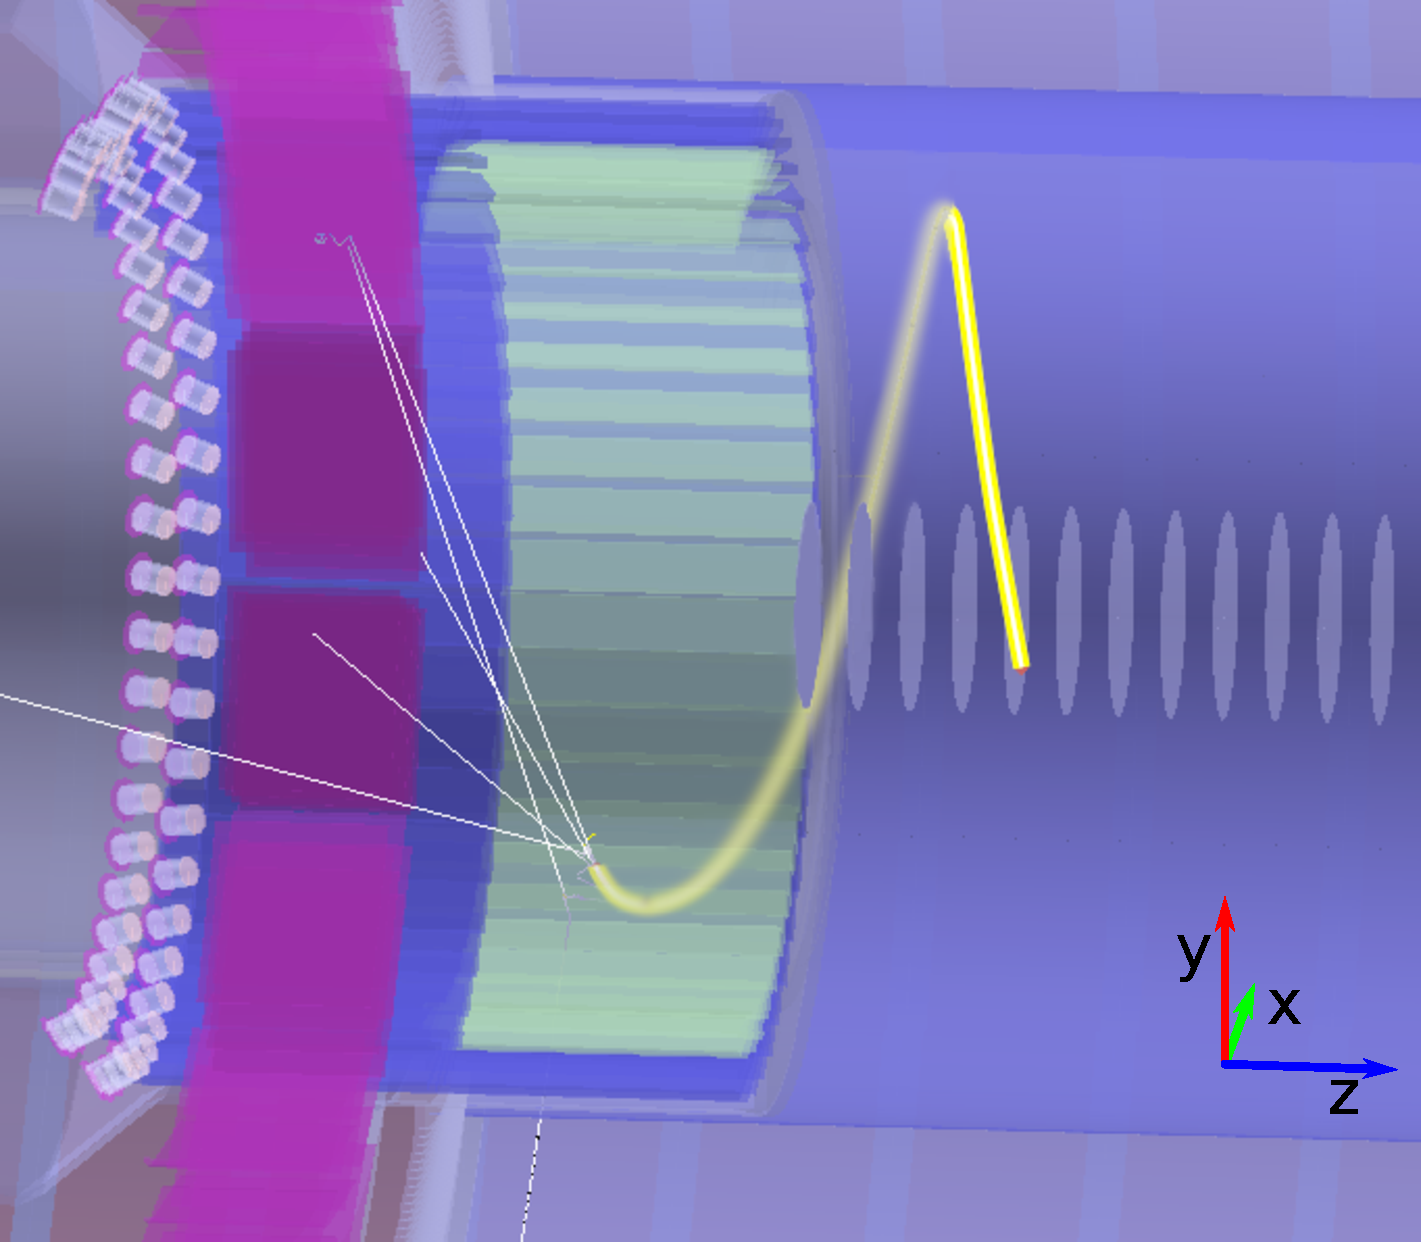
\includegraphics[width=0.85\textwidth]{chapter2/signal_event_display_crop_axes.pdf}
    \vspace{1.18cm}
    \caption{Event shown in \texttt{DisplayCore}, the 3D event display of
    ICEDUST (see Chapter~\ref{ch:software}).}
    \end{subfigure}
    \hfill
    \begin{subfigure}[b]{0.55\textwidth}
    \centering
    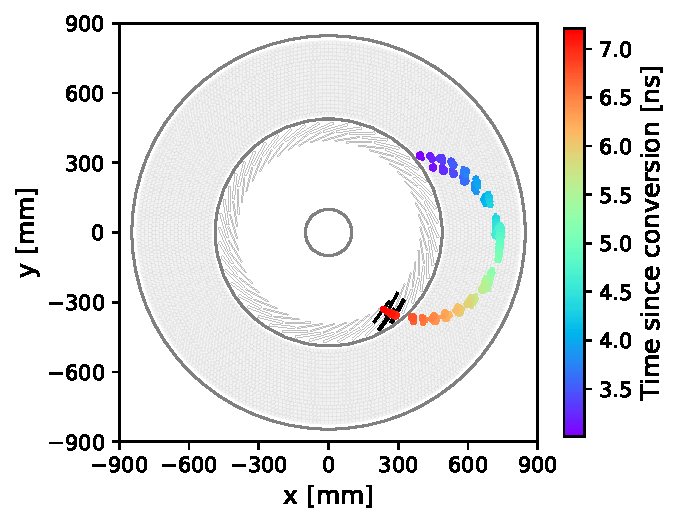
\includegraphics[width=0.99\textwidth]{chapter2/cydet_signal_track_v4.pdf}
    \caption{CyDet event display showing the timing of hits since conversion.}
    \end{subfigure}
    
    \caption{ Conversion electron trajectory as observed by the Cylindrical
    Detector. The effect of stereo angles is visible at the start of the
    trajectory where hits have alternating azimuthal positions around the actual
    electron track. Upon reaching the CTH, the electron produces consecutive
    hits in four adjacent counters, satisfying the fourfold coincidence trigger
    criterion.}
    \label{fig:cydet_signal_event}
\end{figure}


% Timing
The expected timing of conversion electrons is directly related to the time
distribution of muons bound inside the stopping target, shown in
Figure~\ref{fig:timing_distributions}. In Phase-I, in order to suppress prompt
backgrounds from the beam flash, the detector is tuned to only start triggering
on events that occur at least $t=\SI{700}{\ns}$ after each proton collision.
This acceptance criterion retains only \SI{30}{\percent} of all signal events
because the majority of bound muons, having an average lifetime of \SI{864}{\ns},
will have undergone decay or capture before the start of the window.


\section{Experimental backgrounds}\label{sec:backgrounds}

\begin{table}
    \centering
    \begin{tabular}{l|cccc|c}
        \toprule
        Background source & Intrinsic & Stray protons & Antiprotons &
        Cosmics  & Total\\ 
        Estimated events & 0.014 & 0.007 & 0.001 & 0.010 & 0.032 \\ \bottomrule
    \end{tabular}
    \caption{Expected number of background events from each potential
    source~\cite{the_comet_collaboration_comet_2020}. The total count is much
    smaller than one, such that the observation of a single signal electron
    could be evidence that charged lepton flavour is violated.}
    \label{tab:backgrounds}
\end{table}

Intrinsic backgrounds from muon decay-in-orbit and nuclear muon capture can
mimic the conversion signal, as discussed in Section~\ref{sec:sm_backgrounds}.
The COMET experiment is also affected by experimental backgrounds caused by the
intense beam, as well as cosmic ray-induced events.

Beam-induced backgrounds include delayed events caused by slow particles and
products of stray protons arriving between two bunches.
Antiprotons are the main source of delayed backgrounds due to their slow
speed relative to pions and muons of the same momentum. They are negatively
charged so cannot be efficiently selected out by the beamline, hence they can
collide late with the muon stopping target and produce signal-like secondary
electrons during the trigger window.

When a stray proton hits the pion-production target late, secondaries may
quickly travel to the detector region and produce a signal-like electron, which
can also be mistaken for the conversion signal. This is the main reason for
requiring the strict extinction factor $R_\mathrm{extinction}$ of
Equation~\ref{eq:extinction} from the J-PARC proton beam.

Finally, cosmic rays could be a major source of background events. The
background rate depends heavily on the amount of shielding and material above
the COMET detector system, as well as the efficiency of the cosmic ray veto. The
topic of rate estimation for cosmic ray-induced backgrounds is discussed more
thoroughly in Chapter~\ref{ch:cosmics}.



Table~\ref{tab:backgrounds} shows the rates estimated in the COMET Phase-I
technical design report (TDR)~\cite[Section
10.6]{the_comet_collaboration_comet_2020} for each source of background in the
$\mu$--$e$ conversion search. The total number of background events over the
data acquisition run time is predicted to be 0.032 given an extinction factor
$R_\mathrm{extinction} = 3 \times 10^{-11}$. Since this background event count
is much smaller than one, the observation of a single signal-like electron may
suggest that a CLFV process is at play, which would further motivate this search
through COMET Phase-II and beyond.



% Backgrounds = signal contamination. Backgrounds do not enter the equation for
% SES, but SES involves quality cut factors whose purpose is to lower background
% rates. The goal is to show that background rate << 1, only then SES makes
% sense since we've shown that we can actually detect a single event with little
% doubt that it's a conversion signal.


\section{Sensitivity and run time}\label{sec:SES}

The sensitivity of the COMET experiment is conventionally expressed as a
\emph{single event sensitivity} (SES), which is defined as the value of the
$\mu$--$e$ conversion branching ratio for which COMET expects to observe one
event (smaller is better). SES takes into account the net acceptance of signal events by the
detector system, however it does not say anything about the experimental
backgrounds. When using SES as a figure of merit, a study of potential
background sources is usually necessary to show that the expected number of
background events is not greater than one. 

The total number of coherent $\mu$--$e$ conversions produced by a
population of $N_\mu$ bound muons can be expressed as
$$
N_\mathrm{conversion} = N_\mu \cdot \mathcal{B}_\mathrm{conversion} \cdot
\mathcal{B}_\mathrm{capture} \cdot f_\mathrm{coherent},
$$
where $\mathcal{B}_\mathrm{conversion}$ is the conversion branching ratio
normalised to the branching ratio of nuclear muon capture
$\mathcal{B}_\mathrm{capture}$, and $f_\mathrm{coherent}$ is the fraction of
conversions estimated to occur coherently and leave the nucleus in its ground
state.
The number of conversion electrons that will be observed by the detector is then
$N_\mathrm{obs} = N_\mathrm{conversion}\, A_{\mu-e}$, where $A_{\mu-e}$ is the
detector's net signal acceptance. If we require $N_\mathrm{obs} = 1$ and
rearrange to find the corresponding value of $\mathcal{B}_\mathrm{conversion}$,
we obtain the single event sensitivity:
\begin{equation}\label{eq:ses}
\mathrm{SES} \, \equiv \, \mathcal{B}_\mathrm{conversion}^{N_\mathrm{obs}=1}
 = \, \frac{1}{N_\mu \  A_{\mu-e} \  
\mathcal{B}_\mathrm{capture} \  f_\mathrm{coherent}}.
\end{equation}
In COMET Phase-I, the signal acceptance can be broken down into seven efficiency
factors: geometrical acceptance, hardware (trigger and data acquisition), track finding,
track reconstruction quality cuts, momentum window and trigger time window.
Table~\ref{tab:acceptance} lists these factors as they were estimated in the
COMET Phase-I TDR~\cite[Section 10.1]{the_comet_collaboration_comet_2020}. 

\begin{table}
    \centering
    \begin{adjustbox}{max width=1.1\textwidth,center}
    \begin{tabular}{l|cccccc|c}
        \toprule
        Factor & Geometrical & Hardware & Track-finding & Cuts & Momentum
        & Timing & Net
        \\ 
        Efficiency & \SI{26}{\percent} & \SI{81}{\percent} &
        \SI{99}{\percent} & \SI{70}{\percent} & \SI{93}{\percent} &
        \SI{30}{\percent} & \SI{4.1}{\percent} \\
        \bottomrule
    \end{tabular}
    \end{adjustbox}
    \caption{ Efficiency factors used to determine the signal acceptance in the
    COMET Phase-I TDR~\cite{the_comet_collaboration_comet_2020}. The net
    acceptance is the product of all efficiency factors. ``Cuts'' refers to
    track quality cuts, used to reject events with irregular tracks that cannot
    be accurately fitted and reconstructed.}
    \label{tab:acceptance} 
\end{table}

From the net signal acceptance $A_{\mu-e} = \SI{4.1}{\percent}$, we can now
estimate the total data acquisition run time required to reach the sensitivity
goal of the experiment, $\mathrm{SES} = 3\times 10^{-15}$, using
Equation~\ref{eq:ses}. The required number of bound muons is thus $N_\mu = 1.5
\times 10^{16}$. This quantity can be related to the total run time $T$ via the
proton beam current $I_p = \SI{0.4}{\micro\ampere}$ and the yield of stopped
muons per collision $R_{\mu / p} = 4.7\times 10^{-4}$:
$$
N_\mu = T \cdot \frac{I_p}{e} \cdot R_{\mu / p}.
$$
This equation is rearranged for $T$ to yield $T = 146$~days of data acquisition
for a Phase-I SES of $3 \times 10^{-15}$.

%\chapter{Backward Monte Carlo simulation for cosmic ray events}\label{ch:cosmics}

\begin{markdown}

1. Intro to BMC: relation to adjoint MC (find refs), maybe diagram

2. Physics: how we use BMC to determine rates of cosmic events: equations for
flux, sampling PDF, BMC weights, topography map of J-PARC

3. Integration into ICEDUST: implementation of sampling methods, event loop, output to
oaRooTracker format
+ `https://gitlab.in2p3.fr/comet/ICEDUST_packages/-/merge_requests/534`
+ `https://gitlab.in2p3.fr/comet/ICEDUST_packages/-/wikis/Backward-Monte-Carlo-sampling-with-SimBackwardMC#rate-calculation`

3. Actual estimation of background rate in Phase-I, maybe just quoting V's
result


\end{markdown}

% Intro: cosmics are important
Cosmic ray-induced events represent a significant part of the expected
background in the COMET experiment, as discussed in
Section~\ref{sec:backgrounds}. Cosmic muons irradiate the Earth at irregular
intervals and have a wide energy range, hence some fraction of them will be able
to mimic the conversion signal by entering the COMET detector system. 

Estimating the rate at which cosmic muons might produce signal-like events is
computationally expensive through standard Monte Carlo simulation methods. This
is due to the fact that the source of cosmic muons, i.e.\ the atmosphere, has a
much greater spatial extent than the active detector region. Hence, most cosmic
events generated from an atmospheric source will miss the detector completely
and not contribute in the estimation of the background rate, resulting in wasted
computation time.

A reverse (or adjoint) Monte Carlo simulation is one where the flow of particle
transport is reversed, i.e.\ events are generated in the sensitive detector
volume and propagated backward in time until they reach the source. This method
was initially used in 1967 to estimate gamma-ray and neutron radiation doses in
nuclear reactors~\cite{doi:10.13182/NSE68-A19235,doi:10.13182/NSE69-A19116}.
More recently, reverse MC has also been integrated into Geant4
simulations~\cite{DESORGHER2010247} for dosimetry in space, reversing the
electromagnetic physics of electrons, protons and ions.

In the case of muons, a backward transport method was developed by Niess et
al.~\cite{Niess_Barnoud_Carloganu_Menedeu_2018} in the context of muon
tomography, and it was later adapted to the COMET experiment in order to refine
estimations of the background rate from cosmic rays. This chapter discusses the
backward MC method for cosmic muons, how it is applied to COMET and the
resulting rate estimations in COMET Phase-I.


\section{Backward Monte Carlo transport}
In standard Monte Carlo simulations, events are generated by a source and
propagated forward in time according to their equations of motion and
interaction cross-sections within any surrounding medium. In a situation where
the source is large compared to the sensitive detector volume, as illustrated in
Figure~\ref{fig:bmc_configuration}, events have a high probability to miss the
detector and contribute nothing in the desired computation.

In backward MC, events are generated according to an arbitrary probability
density function (PDF) around the detector volume. The overall sampling PDF is
typically the composite of a position, direction and energy sampling
distributions, i.e.\ 
$$
p(\bm{x}, \bm{p}, E) = p(\bm{x}) \times p(\bm{p}) \times p(E),
$$
where $p$ denotes a PDF whose integral is 1, $\bm{x}$ denotes position, $\bm{p}$
direction and $E$ energy. 

\sepfootnotecontent{A}{See Reference~\cite{DESORGHER2010247} for a thorough
discussion of adjoint cross-sections, weights, weight corrections and source
normalisation.}

Each event is propagated backward using adjoint transport and interaction
kernels such that the probability of the event can eventually be determined. At
each step of the propagation, a multiplicative weight is computed from the
adjoint interaction cross-sections in the local medium. When the particle
reaches the source, the directional flux at the source is used as a
normalisation factor to yield the final event weight\sepfootnote{A}. Given a
significant enough sample of reverse events, the weights can be summed to
obtain the absolute flux or rate of particles hitting the detector.


% Interesting paragraph from desorgher:
%  The Monte Carlo sampling of a big enough number of reverse tracks is
%  equivalent to the integration of the weight W over all independent variable
%  (E1,O1,Sd,x1,E0, ...) summed over all type of reverse reactions, atomic
%  elements, adjoint primaries, and adjoint secondaries. In this integration the
%  cases where more than one reaction and no reaction occur are also considered
%  and only the tracks reaching the external source are accounted for. By this
%  way the same answer is obtained as in the forward case.

\begin{figure}
    \centering
    %\includegraphics[width=0.6\textwidth]{chapter5/qwe.png}
    \caption{BMC configuration.}
    \label{fig:bmc_configuration}
\end{figure}

% How does one estimate the rate of cosmics from the sampling PDF and BMC
% weights?
% Describe procedure / maths?

% We backward propagate the same event many times in order to get a reasonable
% rate estimate. Perhaps mention that.

\section{Cosmic muon rate estimation}
% Here, talk about the COMET setup: 
% + We want to estimate the rate of background events caused by 
%   muons+secondaries hitting the detector
% + Thus, we sample muons+/- around the envelope of the CRV, according to [spell
%   out PDF]
% + We apply backward MC up to an atmospheric muon flux model at altitude X,
%   tabulated from CORSIKA etc.
% + We can first estimate the cosmic muon rate on each surface of the CRV
%   Show plots etc.
% + From the events generated at the CRV envelope, it is also possible to
%   propagate forward to determine which events might produce signal-like
%   tracks.
% + Once this is done, we use the results from backward propagation to estimate
%   rate of background-inducing cosmic muons, qed.


% Do we talk about the PUMAS, GOUPIL setup?
% ICEDUST integration?

\chapter{COMET Phase-I sensitivity and backgrounds}

With the framework to simulate backgrounds from atmospheric muons in place, we
can now combine the results into a complete sensitivity and background
simulation study for COMET Phase-I. In this chapter, we discuss our simulation
samples consisting of signal, decay in orbit (DIO), and atmospheric events, and
present our resulting expectations of the performance of Phase-I.

\section{Simulation setup}
Three simulation samples are produced for this study. A $\mu$--$e$ conversion
sample, a DIO sample and an atmospheric muon sample. All three are simulated in
the geometrical world shown in Figure~\ref{fig:bmc_geometry}. This geometry
differs from the older TDR design~\cite{the_comet_collaboration_comet_2020} by
the number of counters in the CTH. Here, each layer of the CTH has 64 counters
instead of the original 48, which mainly affects the detector's geometrical
acceptance. In addition, the outer layer of the CTH is composed of plastic
scintillator counters rather than the Cherenkov counters, as was originally
planned. As we will see, this has an important effect on the detector's ability
to discriminate atmospheric anti-muons from conversion electrons.

\subsection{\texorpdfstring{$\mu$--$e$}{Muon to electron} conversion} 

\subsubsection{Sample}

The signal sample is the most straightforward to produce. We initially generate
primary electrons with energy $E=\SI{104.97}{\MeV}$ uniformly inside the
stopping target disks. Their direction is isotropically distributed, as would be
the case in the conversion process. A uniform position distribution in each disk
is not realistic, because the actual distribution depends on where in the
stopping target the muons in the beam become bound. To account for this, the
events are weighted according to the stopping positions of muons recorded in the
MC5 simulation. The weighting factor is determined from the relative probability
for a muon to stop at the sampled position, which is estimated by histogramming
the stopping positions in each disk.
Figure~\ref{fig:stopping_position_reweighting} shows the sampled uniform
position distribution and the resulting distribution after weighting. In total,
$N_\mathrm{signal} = 2\times 10^6$ events are simulated to compose the signal
sample.

% After applying geom cut of CTH trigger, how many remain?

\begin{figure}
    \centering
    \begin{subfigure}{0.46\textwidth}
        \centering
        \caption{Pre-weighting.}
    \end{subfigure}
    \hfill
    \begin{subfigure}{0.46\textwidth}
        \centering
        \caption{Post-weighting.}
    \end{subfigure}
    \caption{ Initial position distribution of signal electrons before and after
        weighting them by the likelihood of a muon being bound in each bin. }
    \label{fig:stopping_position_reweighting}
\end{figure}

\begin{figure}
    \centering
    
    \caption{Conversion signal event in the CyDet system.}
    \label{fig:signal_in_cydet}
\end{figure}

\subsubsection{Selection}
Signal events are selected based on detector acceptance criteria. We first require
fourfold coincidence in the CTH. The fraction of events remaining
defines the geometrical acceptance 
$$
A_\mathrm{geom} \equiv  \frac{\text{fourfold coincidences}}{N_\mathrm{signal}}.
$$
In our simulation setup with the 64-counters-per-layer CTH, our estimated
geometrical acceptance is $A_\mathrm{geom} = \SI{21}{\percent}$. In comparison,
the TDR cites $A_\mathrm{geom} = \SI{26}{\percent}$ with the previous design of
the CTH. 
\hl{Figure~X shows a conversion event which passes the
fourfold coincidence selection criterion.??}

% Reconstruction
We do not fully simulate the reconstruction of signal electron trajectories in
the CDC. In order to approximate the effect of reconstruction uncertainties, a
smearing is applied to the true momentum of each track. The reconstructed
momentum is estimated as $p_r = p_t + x$, where $p_t$ is the true momentum of
the electron as it enters the CDC, $x \sim \mathcal{N}(0, \sigma)$, and $\sigma
= \SI{200}{\keV/\clight}$ is the expected momentum resolution of the CDC.

% Other acceptance factors (not simulated)
Other acceptance criteria, such as the trigger timing window and reconstruction
quality cuts, are not properly simulated in this study. Instead, we apply
efficiency factors for each of them based on their TDR estimates.
\hl{Reference a table here?}


\subsection{Muon decay in orbit}
\subsubsection{Sample}
The DIO sample is similar to the signal sample in that the initial position
of signal and DIO electrons is identically distributed. Hence, we also sample
uniformly in the stopping target disks and then weight the events according to
the MC5 stopping position distribution. Similarly, the direction of DIO
electrons is sampled isotropically. The energy distribution is thus the only
difference between the two samples. 

\begin{figure}
    \centering
    
    \caption{Energy spectrum of DIO electrons from muonic aluminium atoms.}
    \label{fig:czarnecki_spectrum}
\end{figure}

The theoretical energy spectrum of DIO electrons produced in aluminium muonic
atoms was determined by Czarnecki et al.~\cite{czarnecki} and is shown in
Figure~\ref{fig:czarnecki_spectrum}. Their calculated spectrum is used to
determine an energy weighting factor for simulated DIO events. In a similar way
to the position weighting procedure, DIO events are first generated with a
uniform energy distribution, and then weighted according to the relative
likelihood for a DIO electron to have the sampled energy.
Figure~\ref{fig:dio_energy_reweighting} shows the weighted energy distribution
compared to the theoretical energy spectrum. \hl{FIGURE and then adjust text}.
The DIO sample is composed of $N_\mathrm{DIO} = 10^7$ events in total.

\begin{figure}
    \centering
    
    \caption{DIO-induced background with momentum  $p=\SI{1}{\MeV/\clight}$.}
    \label{fig:muon_dio_in_cydet}
\end{figure}

\subsubsection{Selection}
The selection of DIO events is identical to the selection of conversion events.
We require a fourfold coincidence in the CTH, and then apply a Gaussian smear to
the true momentum of the electron to simulate track reconstruction. The same
efficiency factors as for signal events are applied.

\subsection{Atmospheric muons}

\subsubsection{Sample}

Atmospheric muon events are simulated as explained in
Section~\ref{sec:cosmic_event_sampling}. Two samples are produced, one on the
entire surface of the CRV and one more densely concentrated on its upstream and
downstream openings. Because of how rarely a sampled atmospheric event produces
signal-like features, the atmospheric dataset is by far the largest of the
three, with $1 \times 10^9$ events generated on the envelope and $1.4 \times
10^9$ on the openings.



\begin{figure}
    \centering
    
    \caption{Cosmic ray-induced background with momentum $p=\SI{1}{\MeV/\clight}$.}
    \label{fig:cosmic_bg_in_cydet}
\end{figure}


\hl{TODO remove below}

The time distribution of signal, DIO and atmospheric events is not realistically
simulated in this study. Instead, we apply an average timing window efficiency
factor to all events in order to estimate the total count integrated over
data-acquisition time.

The time efficiency factor is not the same for signal, DIO and cosmics,
because they don't have the same time distribution. For cosmics, the time
distribution is ~uniform, so the factor should just be live time / (live +
dead time). For signal and DIO, it is dependent upon the time distribution of
muon bound in the tgt.

\subsubsection{Selection}
\hl{TODO}


\subsection{Sample weighting}
\sepfootnotecontent{fn:conv_br_norm}{The nuclear muon capture branching ratio appears in this
expression because the branching ratio of $\mu$--$e$ conversion is
conventionally normalised to $\mathcal{B}_\mathrm{capture}$.}

Because they originate from different processes, the three MC samples must be
weighted differently in order to determine the absolute contribution from each.
The conversion and DIO processes both originate from the muons bound in the
stopping target, hence we can express the total number of expected conversion
and DIO electrons in terms of the total number of stopped muons $N_\mu$.
The number of signal electrons, as a function of the conversion branching
ratio $\mathcal{B}_\mathrm{conversion}$, is:
$$
N_{e^-}^\mathrm{conversion} = 
N_\mu \, \mathcal{B}_\mathrm{conversion} \, 
\mathcal{B}_\mathrm{capture} \, f_\mathrm{coherent},
$$
where $\mathcal{B}_\mathrm{capture} = 0.61$ is the branching ratio of nuclear
muon capture\sepfootnote{fn:conv_br_norm} and $f_\mathrm{coherent}=0.9$ is the
fraction of conversions that are coherent. Similarly, the total number of DIO
electrons can be expressed as:
$$
N_{e^-}^\mathrm{DIO} = N_\mu \, \mathcal{B}_\mathrm{DIO},
$$
where $\mathcal{B}_\mathrm{DIO} = 1 - \mathcal{B}_\mathrm{capture} -
\mathcal{B}_\mathrm{conversion} \approx 0.39$ is the branching ratio of DIO.


In the case of atmospheric muons, the backward MC procedure yields an absolute
rate. This rate is multiplied by the total data acquisition (DAQ) time of the
experiment to obtain the expected background count:
$$
N_\mathrm{atmospheric} = R \times T_\mathrm{DAQ},
$$
where $R$ is the total atmospheric background rate, and we set
$T_\mathrm{DAQ}=146$ days, corresponding to $N_\mu = 1.5\times 10^{19}$, in this
study. 

\subsubsection{Trigger time window efficiencies}
In order to take into account the trigger timing window, we assume that
atmospheric muons irradiate the detector with a uniform time distribution.
Hence, the time window efficiency factor is simply the average fraction of
time when the trigger is active:
$$
\epsilon_\text{time window}^\mathrm{atmospheric} =
\frac{8}{9}\,\frac{1170 - 700}{1170} = \SI{36}{\percent}
$$
assuming the trigger window is between 700 and \SI{1170}{\ns}, and where the
factor $\frac{8}{9}$ arises from the bunch structure of the J-PARC main ring. In
contrast, the efficiency factor for conversion and DIO electrons
$\epsilon_\text{time window}^\text{conversion|DIO} \approx \SI{30}{\percent}$ is
smaller because the time distribution of bound muons peaks around \SI{300}{\ns},
before the trigger becomes active (see Figure~\ref{fig:timing_distributions}).



\section{Single event sensitivity}
The single event sensitivity (SES) is defined as the value of the $\mu$--$e$
conversion branching ratio required for the experiment to observe one signal
event. It can be expressed in terms of the experimental acceptance $A_{\mu-e}$ and the
total number of muons stopped in the stopping target $N_\mu$:
\begin{equation}
    \mathrm{SES} = \frac{1}{N_\mu\,A_{\mu-e}\,\mathcal{B}_\mathrm{capture}\,f_\mathrm{coherent}},
\end{equation}
where $\mathcal{B}_\mathrm{capture} = 0.61$ is the branching ratio of nuclear
muon capture and $f_\mathrm{coherent} = 0.9$ is the fraction of conversions
expected to leave the nucleus in its ground state.

% Is it worth ELI5 here?
% The net signal acceptance $A_{\mu-e}$ is the product of various factors stemming
% from the experiment's design and inefficiencies in the processing,
% reconstruction and selection of candidate events. 

% How do we approach the fact that CTH geom has changed so our geom acceptance
% is lower?

\hl{ v We've already mentioned trigger selection and acceptance in the Selection
    subsec of every sample. Cut.}
    
In this study, the CTH trigger mechanism was simulated by finding events
involving a fourfold coincidence. The fraction of signal events which induce a
trigger is defined as the geometrical acceptance $A_\mathrm{geom}$. In our
simulation setup, the CTH contains 64 counters per layer, two layers
in each module, one module at the upstream end of the CDC and the other
downstream (256 counters in total). Our estimated geometrical acceptance is
$$
A_\mathrm{geom} \equiv \frac{\text{fourfold coincidences}}{N_\mathrm{signal}} = \SI{21}{\percent}.
$$
In comparison, the COMET Phase-I TDR~\cite{the_comet_collaboration_comet_2020}
cites $A_\mathrm{geom} = \SI{26}{\percent}$ with the previous design of the CTH,
which had 48 counters per layer. This reduced acceptance worsens the sensitivity
of the experiment slightly. In this study, none of the other experimental
aspects that contribute to the net acceptance were changed, hence we use the
other factors of $A_{\mu-e}$ from the TDR, and only replace the value of
$A_\mathrm{geom}$ with the newly estimated one. Values of the acceptance
coefficients used in our study are shown in Table~\ref{tab:acceptance}. The net
signal acceptance using these factors is $A_{\mu-e} = 0.032$.

The number of muons stopped in the stopping target, $N_\mu$, is a function of
the COMET beam power, the target material, the design of the
transport system, and the total data-acquisition time. 
The target material sets the yield of
backward-going pions which will decay to muons of the right momentum to come at
rest in the muon stopping target. This, combined with the transport system,
determines the yield of stopped muons per proton collision $R_{\mu/p} \equiv
\frac{\text{muons stopped}}{\text{proton on target}}$. Here, we use the
MC5 dataset, a sample of $10^9$ POT collisions, to estimate $R_{\mu/p}=4.86
\times 10^{-4}$.
The beam power and data-acquisition time together determine the total number of proton
collisions that will occur. COMET Phase-I requires $N_\mathrm{POT} = 3.15 \times
10^{19}$ collisions in order to reach its sensitivity goal, corresponding to a
data-acquisition time of $T=146$ days.
These figures allow us to estimate the total number of stopped muons
$$N_\mu = R_{\mu/p} \times N_\mathrm{POT} = 1.56\times 10^{16},$$
which can be substituted into the SES formula:
\begin{equation}\label{eq:my_ses}
\mathrm{SES}
=\frac{1}{N_\mu\,A_{\mu-e}\,\mathcal{B}_\mathrm{capture}\,f_\mathrm{coherent}}
= 3.81\times10^{-15}.
\end{equation}
This value is slightly worse than the TDR estimation,
$\mathrm{SES}_\mathrm{TDR}=3\times 10^{-15}$, because of our lower geometrical
acceptance when using the new CTH design.

% \begin{table}
%     \centering\begin{tabular}{l|ccc}
%         \toprule
%         a&b&c&d\\\midrule
%         a&b&c&d\\
%         \bottomrule
%     \end{tabular}
%     \caption{ Acceptance coefficients used to estimate the single event
%     sensitivity in Equation~\ref{eq:my_ses}. These also apply to the
%     decay-in-orbit background rate estimation. }
%     \label{tab:ses_efficiency_factors}
% \end{table}


\section{Momentum spectra}
Because the signal has a clear mono-energetic signature, a precise measurement
of the momentum of candidate tracks helps to discriminate signal from
backgrounds. Figure~\ref{fig:log_spectrum} shows the momentum spectrum
for candidate conversion, DIO and atmospheric events.

\begin{figure}
    \centering
    
    \caption{Log spectrum.}
    \label{fig:log_spectrum}
\end{figure}

\section{Discussion}

\subsection{Atmospheric $\mu^+$ backgrounds}

\subsection{CRV efficiency}

\subsection{Particle identification}

\chapter{Discussion}
\label{ch:discussion}

This thesis presents two main original contributions: we designed a fake Monte
Carlo data generator for the CDC using machine learning, and we estimated the rate of
atmospheric muon backgrounds in the COMET Phase\nobreakdash-I $\,\mu$--$e$ conversion search
using a backward MC simulation technique. In this chapter, we discuss our main
findings, the limitations we encountered and ideas toward future studies on
either topic.

\section{Data augmentation with machine learning}

\subsection{Summary}
The CDC GAN, discussed in Chapter~\ref{ch:gan}, provides a way to produce
synthetic Monte Carlo data in the Cylindrical Drift Chamber. The design of this
generative algorithm is based on Generative Adversarial Networks, a technique
which is more and more widely used in HEP and in other domains to produce fake
samples by learning from an existing dataset of real samples. The CDC GAN is
trained on MC-simulated hits using the WGAN-GP algorithm. Its discriminator and
generator are convolutional neural networks that can process ordered sequences
of hits, which allows the GAN to learn both from per-hit features, and from the
relations between multiple consecutive hits. Once trained, the GAN is evaluated
in multiple ways. Firstly, the distributions of the synthetic data are compared
to those of the training dataset. In addition, we investigated quality metrics,
which typically involve an external performance criterion implemented by a third
neural network trained independently. These evaluation methods allow us to
determine which aspects of the training data are adequately modelled by the GAN,
and where there are discrepancies. This then helps to guide the design of the
model to increase the quality of generated samples.

% Interpretation
After training, the CDC GAN provides a way to produce original hit data at least
six orders of magnitude more quickly than by means of traditional MC simulation,
using GPUs. We are therefore able to generate large samples of background events
very efficiently. This can be useful, for instance, in studies which require a
pure signal sample to be overlaid onto an ambient background, e.g.\ to optimise
a hit filtering algorithm. Alternatively, GAN-generated data can serve to
compose a mock dataset, combining signal events with all sources of backgrounds
into one large-scale simulation sample used to test the readiness of our
data-processing chain prior to the data acquisition period.




The CDC GAN design and architecture are generalisable to other detector systems
that have discrete elements. For instance, the CTH is somewhat analogous to the
CDC if we treat the scintillation counters like the cells of the CDC. One
difference is that distance of closest approach (\texttt{doca}) has meaning for
CDC hits but not for CTH hits. Although it is not discussed in detail in this
thesis, a CTH GAN prototype was developed based on this analogy, with the
\texttt{wire} feature acting as the counter index, and the
\texttt{doca} feature removed. Based on early evaluations, we observed similar
performance and sample quality as exhibited by the CDC GAN.




% Limitations
\subsection{Limitations and recommendations}
\subsubsection{Training data preselection}
The CDC GAN is only trained on a restricted part of the CDC hit data.
Reconstructible tracks, defined by their momentum $p>\SI{50}{\MeV/\clight}$, are
removed from the training dataset in order to prevent the model from generating
patterns that are too similar to the conversion signal without the proper
associated truth information. Unlike high-momentum tracks whose source
(conversion, DIO, RMC, etc.) matters in studies of the experimental outcomes,
the origin of low-momentum tracks is typically irrelevant, hence those hits can
be grouped into one large ``noise'' category. The GAN then learns only from hits
in that category, and all GAN-generated data can safely be labelled as noise as
well. However, training on a subset of hit data prevents us from using the GAN
to generate an entire background dataset: the GAN must be complemented by real
MC hits of reconstructible tracks, which is computationally expensive to
produce. 

Training a conditional GAN~\cite{Mirza2014ConditionalGA} with the ability to
generate labelled hits was considered. However, the concern that the model would
be unable to grasp the physical laws at play in the hit patterns of
high-momentum particles was too great, hence this solution was discarded. In a
future study, a physics-informed conditional GAN, where the dynamics of charged
particle transport in a magnetic field are encoded into the discriminator in
order to regulate the generator, could be considered to build a universal
background hit generator.

\subsubsection{Feature representation}
One of the difficulties in designing the GAN was in determining the best way to
handle the discrete feature, wire index. Multiple methods were considered, such
as using actual or transformed wire positions as a real-valued feature, or using
a trainable embedding matrix to make the GAN learn its preferred representation
of the geometry. Eventually, we chose to represent the wire index as a one-hot
encoded vector and use a matrix of wire positions to assist the model in
locating wires, since that yielded the most faithful results. However, this
aspect of the GAN design appears to be one of the major quality-limiting factors
because of the large dimensionality of this one-hot vector compared to the other
features. 

A better design would be achieved by representing the wire index as a
low-dimensional quantity while informing both networks of the location of hits,
however a way to fulfil both requirements at once was not found in our
investigations.

\subsubsection{Hit sequence arrangement}

In order to train the GAN as efficiently as possible, we arrange hits from
multiple particles together into fixed-length sequences that can be processed
quickly convolutional layers. This arrangement is not physical: unrelated hits
from different particles become neighbours in the sequence. When processed by a
convolution kernel, consecutive hits will be treated as if there was some
relationship between them (as for neighbour pixels on an image), but this is
sometimes false. This leads the GAN to learn patterns that are artificial and
only the product of our arrangement. 

Keeping hits from different tracks separate would most likely yield a better
model of the underlying tracks. However, it would also prevent the networks from
being built with convolutional layers. Techniques developed and used in natural
language processing, such as transformers~\cite{10.5555/3295222.3295349}, could
be applied here to build a model that can process variable-length hit sequences
(in analogy with sentences) while remaining efficient to train.


\subsubsection{Quality evaluation}

Evaluating samples generated by the CDC GAN is inherently difficult. Unlike
visual or audio data, one cannot precisely estimate the sample quality
perceptually. Hence, in Section~\ref{sec:gan_eval}, we compare feature
distributions and use KL divergence and more complex metrics to define a
quantitative measure of sample quality. Although these methods help in refining
the GAN architecture and in tuning training parameters, no metric can affirm
that the generated data is physical enough to be used to study the experiment
and its outcomes. This is in part due to the fact that the GAN generates
unlabelled hits from the broad category of ``noise'', hence one can only hope to
determine if generated hits belong in that category, or not.

One option could be to condition the GAN~\cite{Mirza2014ConditionalGA} on
particle type and momentum. If the model is able to generate a sequence of hits
based on a prompt, such as ``electron with $p=\SI{15}{\MeV/\clight}$'', then it
becomes easier to verify whether the hit sequence is faithful to the prompt by
comparing to real samples of a similar description \emph{and} by checking that
the physical rules are respected (e.g.\ track curvature, total energy deposit,
etc.). Of course, conditioning comes at the cost of a more complex network
design and training procedure.



\section{Atmospheric muon backgrounds}

\subsection{Summary}
In Chapter~\ref{ch:cosmics}, we presented the backward Monte Carlo simulation
principle, method, validations, and results when applied to the COMET Phase\nobreakdash-I
setup. Backward MC consists in the time-reversed transport of particles from a
volume of interest to a source where the flux is known. Since events are
generated arbitrarily near the volume of interest, this provides a way to focus
computational resources on important events. In this study, we used backward MC
transport of atmospheric muons in order to determine the rate of cosmic
ray-induced backgrounds in the $\mu$--$e$ conversion search. Events are
generated from the surface of the Cosmic Ray Veto in Phase\nobreakdash-I and transported to
a \SI{1600}{\metre}-high atmospheric plane where a pre-computed flux model is
sampled. The flux estimated at the surface of the CRV is then compared with
experimental data from the BESS-TeV and Kiel-DESY spectrometers in order to
validate that the backward sampling yields realistic results. 

Then, in Chapter~\ref{ch:phase-I_study}, we combine the BMC method with a
$\mu$--$e$ conversion sample and a DIO sample in order to determine how each
process contributes in the event counts recorded during the Phase\nobreakdash-I data
acquisition run. The analysis of signal events yields our estimate of the single
event sensitivity of the COMET Phase\nobreakdash-I experiment. Integrating over the entire
run time of Phase\nobreakdash-I, we find that atmospheric muon backgrounds outnumber the
next largest source of background, DIO, by an order of magnitude or more
depending on the exact conditions. The main factor in eliminating atmospheric
backgrounds is the efficiency of the CRV, followed by the CyDet system's ability
to distinguish between electrons and muons. In the absence of a
particle-identifying Cherenkov layer in the CTH, our results summarised in
Table~\ref{tab:bg_summary} suggest that the background count is at least 0.48
over 146 days, versus one signal event assuming $\mathcal{B}_\mathrm{conversion}
= 3.6 \times 10^{-15}$. With the final-stage CTH layout, the background count
falls to 0.08 assuming a \SI{99}{\percent} $\mu^\pm$ identification rate.

% Implications

% Use vs literature? Actually didn't do a lit review here in HEP...
Backward MC simulation is a powerful tool which enabled us to determine that
extremely rare conversion-like events can be produced by atmospheric muons
sneaking into the COMET detector system. These events can be an important
obstacle for the COMET Phase\nobreakdash-I conversion search if no additional way to
reject them, such as particle type identification, is put in place. Using a
standard MC simulation where events are generated far from the detector system,
those rare events that get past the CRV and produce signal-like tracks would
most likely not appear at all in the sample. Hence, the backward MC method is
absolutely key in this study and should continue to prove useful in COMET toward
Phase\nobreakdash-I and Phase\nobreakdash-II. More generally, any experiment searching for rare
processes and which is susceptible to cosmic ray-induced backgrounds will also
benefit from using backward MC to identify the kinds of atmospheric events that
are likely to mimic their signal, and estimate their frequency.

\subsection{Limitations and recommendations}


\subsubsection{Backward transport}
In our study, we used backward MC simulation to transport muons from the surface
of the CRV to the atmospheric plane. The assumption associated with this
procedure is that the muon is able to travel all the way from the atmospheric
source to the surface of the CRV. In reality, this assumption does not
necessarily hold and there is expected to be some fraction of atmospheric muons
which will interact close to the CRV and whose products will induce a background
event. These events do not contribute toward our results. Therefore, we are
underestimating the background rate from cosmic rays, but by how much is
difficult to determine. 

This bias could be addressed by sampling the muons not at the surface of the
CRV, but a little farther away. However, doing so would lead to more events
missing the detector, as is the case in forward MC, and therefore to wasted
computation. Already, in our study, very few sampled events pass the CyDet
selection criteria: around 1 in $10^5$ in the envelope sample, 1 in $10^7$ for
sneaking events. Pushing the sampling surface outward would decrease these
ratios and reduce our statistics further. Nevertheless, it can be done in the
future in order to estimate the extent of the bias.

\subsubsection{Sampling distributions}

Atmospheric muons are sampled around the CRV with arbitrary energy and direction
distributions. Our selection shows that only one event in \num{100000} produces
a fourfold coincidence and a track in the CyDet system. In a future iteration of
this study, one could determine if there is some region of the sampling phase
space which never contributes to the selected events: perhaps very high or very
low energy events, or events which are incident upon the CRV within a specific
range of azimuthal or zenith angle. Eliminating this region of phase space from
the sampling distribution function would increase the fraction of simulated
events which pass the selection, thus increasing the statistics on events of
interest for the same computational cost.


\subsubsection{Event selection}

To identify background candidates, events are selected that have a fourfold
coincidence in the CTH and an associated track in the CDC. When reconstructing a
trajectory, the track fitting algorithm ignores hits produced by other particles
in the CDC during the same event. Instead of using a track finding algorithm, we
use truth information from the MC simulation in order to select hits from the
right particle and provide them to the track fitting function. This has caused
at least one known inaccuracy in our study: events where a high energy muon
produces a shower in the CDC sometimes induce a fourfold coincidence, thus they
pass our selection criteria and may be counted as background events. In
realistic conditions, events that suddenly saturate a large fraction of CDC
channels, such as a high-energy shower, will most likely be discarded because
tracks cannot be reconstructed from the event. Therefore, these should not have
been counted as part of the integrated background, for instance in
Figures~\ref{fig:log_spectrum_nocuts} and~\ref{fig:bg_count_vs_crv_efficiency}.
These high energy muons typically fly straight through the CyDet system and hit
the CRV along the way. Hence, although this issue in our selection is likely to
have caused a slight overestimation of the total background rate, we expect the
sneaking component to be unaffected.

\subsubsection{Reconstruction and detector response}
Various aspects of our study are not faithful to the actual conditions of
Phase\nobreakdash-I. On the reconstruction side, for the atmospheric muon sample, we use a
helix fit to reconstruct the trajectory of each event where a fourfold
coincidence is produced. During data acquisition, a more complex fitting
algorithm, based on Kalman filtering, will be used. Similarly, for the
conversion and DIO samples, we do not perform reconstruction but naively
smear the true momentum of the track using the design momentum resolution of the
CDC. Because of those simplifications, we expect the resulting momentum spectra
to differ slightly in the real conditions of Phase\nobreakdash-I. 

Although ICEDUST has the capability to fully simulate each sub-detector's
response to incoming energy deposits, digitisation and calibration were not
simulated in this study. Instead, we simplified those processes by applying a
hardware efficiency factor to all samples. Similarly, the timing of events is
also disregarded in our simulation. Instead of assigning a realistic time of
production to conversion, DIO and atmospheric events, and then selecting events
that occur in the trigger time window, we apply an efficiency factor to each
sample based on their expected time distribution and the start and end time of
the trigger window. 

Hence, our study makes use of estimates based on other studies within the
collaboration, rather than conducting fully realistic calculations in the
detector response and reconstruction aspects. In future studies, and as
the Phase\nobreakdash-I data acquisition period approaches, it will be
especially important to rigorously simulate these effects to assess the
performance of the experiment as accurately as possible.

% \section{Mock data composition}
% Generative algorithms and backward Monte Carlo could in principle be combined to
% compose mock datasets. Consider a mock data challenge where one signal event is
% inserted into a large background sample, and the goal is to find this single
% event among the noise. 
% The mock dataset should contain a realistic mix of hits from all sources of
% background. 
% % Beam
% Beam-induced hits can be produced with a hybrid approach mixing GAN-generated
% hits with MC-simulated reconstructible tracks
% % Cosmic
% For atmospheric-induced hits, 
\chapter{Conclusion}

% Muon and LFV
Since the discovery of the muon in 1937, our understanding of its properties has
been steadily evolving. Today, although it fits nicely into the Standard Model
of particle physics, some questions remain standing, and recent tensions
observed between theory and experiment are suggesting that the SM does not give
a complete picture of the muon's underlying nature. Charged lepton flavour
violation is one of the ways in which Nature might deviate from the SM. If CLFV
were observed, it would be a clear indication of new physics. Neutrino-less
muon-to-electron conversion is one of the most sensitive channels to search for
CLFV as its signature is a mono-energetic electron with few sources of potential
backgrounds. According to theoretical constraints, this process ought to be
suppressed beyond experimental sensitivities. Therefore, any observation of the
$\mu$--$e$ conversion signal would yield clear evidence for CLFV and hence guide
the field toward a better understanding of physics beyond the Standard Model.

% COMET
The COMET Phase\nobreakdash-I experiment will soon start its data acquisition
run toward the search for muon-to-electron conversion in aluminium. It is
expected to be a hundred times more sensitive to $\mu$--$e$ conversion than the
previous best measurement by SINDRUM II. To achieve this sensitivity, COMET
Phase\nobreakdash-I will produce an intense pulsed muon beam directed toward an
aluminium target to create muonic aluminium atoms, from which conversion
electrons may emerge. The Cylindrical Detector, which surrounds the muon
stopping target, is designed to clearly identify conversion electrons while
rejecting as many experimental backgrounds as possible. 

% Software & sim
In order to cover the needs of the experiment in terms of simulation,
calibration, reconstruction, data formats and data analysis, the COMET
collaboration develops a comprehensive set of software utilities named ICEDUST.
The work presented throughout this thesis relies heavily on Monte Carlo (MC) data
produced by ICEDUST's {\sc Geant4} simulations of Phase\nobreakdash-I.
% Here is a good place to kind of introduce the problem of producing large-scale
% datasets and estimating atmospheric backgrounds
MC simulations allow us to study the experiment outcomes and to optimise its
design before assembly. However, they are computationally expensive and
typically only allow us to simulate a small fraction of the amount of data
expected to be collected. Additionally, traditional MC sampling is particularly
inefficient when the source of events is far from the detector system, as is the
case when considering cosmic ray-induced backgrounds. This thesis aims to
address these two limitations by partially circumventing the brute force MC
method.

% GAN
We investigate a novel approach to the mass-production of simulation data based
on Generative Adversarial Networks. We propose a neural network generator of
hits for the Cylindrical Drift Chamber, which can produce synthetic energy
deposits in the detector at a rate $10^6$ times higher than the ICEDUST
simulation. The machine learning model is trained on a sample of simulated hits
and learns from their features and relationships. The trained model allows us to
generate only a subset of the hits produced by MC simulation, but far more
efficiently than was previously achievable. Our ambition for this work and
future developments is to enable the production of entire mock datasets, which
can be used by the collaboration in anticipation of data acquisition runs.

% BMC & background study
Additionally, we present a study of the backgrounds caused by cosmic ray-induced
atmospheric muons in the COMET Phase\nobreakdash-I muon-to-electron conversion search. We
use a backward Monte Carlo simulation method to efficiently estimate the flux of
atmospheric muons near the detector system. We then perform a full analysis of
the event count contributions from $\mu$--$e$ conversion, muon decay-in-orbit,
and atmospheric muons. Our findings suggest that an efficient rejection of
atmospheric backgrounds by the Cosmic Ray Veto, combined with particle-type
identification by the Cylindrical Detector, are necessary for the Phase\nobreakdash-I search
to succeed. Under optimistic conditions, namely with a
\SI{99.99}{\percent}-efficient CRV and \SI{99}{\percent} muon identification
rate by the CyDet, we expect 0.08 atmospheric background events during the 146
days of data acquisition. According to our analysis, during this run time, COMET
Phase\nobreakdash-I will be able to achieve a single event sensitivity of $3.61 \times
10^{-15}$.


% Wrap up: what do my results mean for COMET!!!
Our most important contributions have been integrated into the main ICEDUST
software repository and documented for others to use and build upon. As the
COMET experiment goes into the Phase\nobreakdash-I measurement period, we hope that these
techniques will help to refine our understanding of the data and that they can
be applied in preparation for Phase\nobreakdash-II and beyond.
\appendix
\chapter{Integration of backward Monte Carlo software into
ICEDUST}
\label{app:bmc_integration}

% \begin{itemize}
%     \item External packages: PUMAS, GOUPIL, GOUPIL components. Cite~\cite{NIESS2022108438}.
%     \item Internal package: SimBackwardMC
% \end{itemize}


\section{Original implementation}
The backward Monte Carlo simulation software was originally written and applied
to the COMET Phase\nobreakdash-I experiment by Valentin Niess, author
of~\cite{Niess_Barnoud_Carloganu_Menedeu_2018,NIESS2022108438}.
Figure~\ref{fig:pumas_integration_strategy} shows the layout of the original set
of software layers used to run backward MC simulations in the Phase\nobreakdash-I world. 

At the core of the backward Monte Carlo simulation is the backward transport
engine, PUMAS~\cite{NIESS2022108438}. PUMAS is responsible for the propagation
of particles through matter and the computation of MC weights based on the path
taken and the interactions undergone, as discussed in
Section~\ref{sec:bmc_method}. Because it is designed exclusively for this
purpose, PUMAS does not provide utilities for navigating through complex
geometries or sampling the flux from pre-computed tables. Another package,
GOUPIL, takes on this role as an interface to PUMAS, and allows the user to
specify a geometry, a source flux, as well as the local topography and
geomagnetic field around the experiment's location. An additional interface
between GOUPIL and {\sc Geant4}, \texttt{goupil-geant4}, was developed to allow
the user to control backward MC runs with the {\sc Geant4} macro user interface
and to load and navigate the geometry from a GDML file. The final layer,
\texttt{resample-simg4}, provides a command-line interface and enables events
generated by \texttt{SimG4} to be read as input for the backward MC simulation
to estimate their flux.


\begin{figure}
    \centering
    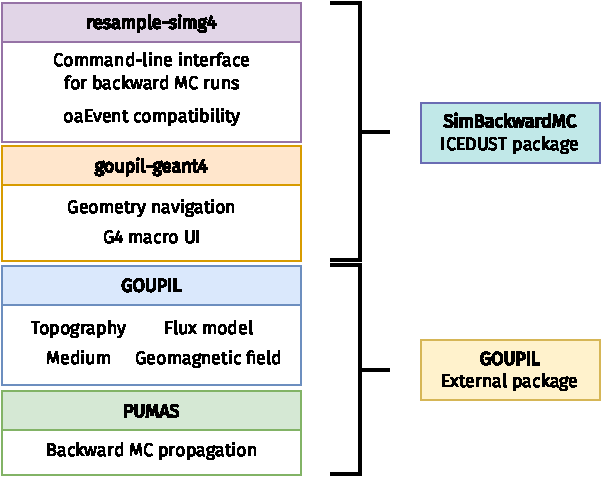
\includegraphics[width=0.6\textwidth]{appendixA/integration_strategy.drawio.pdf}
    \caption{ Software packages that compose the original backward MC simulation
        stack for the Phase\nobreakdash-I study, and organisation of their integrated
        ICEDUST counterparts.}
    \label{fig:pumas_integration_strategy}
\end{figure}

\section{Integration}

Figure~\ref{fig:pumas_integration_strategy} also shows how the original software
was arranged to become part of the ICEDUST framework. Since the PUMAS and GOUPIL
packages are unlikely to undergo quick iterative changes over time, they are integrated
into an external package. The functionalities of the upper two layers of the
stack are combined into a new ICEDUST package called \texttt{SimBackwardMC}.

The way in which the layers are organised is not the only difference between the
original and current software. Three major changes were implemented during the
integration in order to bring the original software closer to the ICEDUST
workflow.

\begin{itemize}
    \item {\bfseries Geometry format:} originally read from GDML files, the
    geometry is now created from the same classes and macro files that define
    the simulation world in forward MC runs by the \texttt{SimG4} package. This
    additionally ensures that the geometry used in forward and backward MC
    simulations is identical.
    \item {\bfseries Entry point:} the main \texttt{resample-simg4} entry point
    was previously a Lua script executed via LuaJIT which defined the
    command-line interface, configured the backward simulation run, and
    processed the output. \texttt{SimBackwardMC} uses a standard ICEDUST event
    loop executable as its entry point to handle command-line arguments, read
    events from input \texttt{oaEvent} files and output the results of the
    backward simulation.
    \item {\bfseries Output format:} \texttt{resample-simg4} wrote the results
    of backward sampling to a text file in a format similar to CSV.
    \texttt{SimBackwardMC} writes to a \texttt{RooTracker} file instead, since
    that is a standard ICEDUST format and a good fit to store the kinematics of
    processed events along with their estimated flux.
\end{itemize}

The integrated backward MC software presented here was used to obtain the
results of Chapters~\ref{ch:cosmics} and~\ref{ch:phase-I_study}. It is also
currently being used in the work of others, for instance to estimate the
atmospheric muon flux at various locations around the Phase\nobreakdash-I detector system
and validate the results with real measurements. Through our standardisation of
some parts of the original software and the addition of specific documentation,
we hope that the \texttt{SimBackwardMC} package will remain a readily accessible
tool for future cosmic ray studies in COMET.


\printbibliography

% \listoffigures
% \listoftables

\end{document}
